\section{Počítání}
\label{sec:pocitani}

V této kapitole se naučíme počítat; a ne, doteď jste to neuměli. Snad všech\-ny
potěšíme, když zvěstíme, že tahle je kapitola je již skutečným úvodem do
problematiky \emph{diskrétní matematiky}. Otázky typů \uv{Kolik je čeho?},
\uv{Kolika způsoby mohu něco udělat?} skutečně nikam jinam patřit ani nemohou,
protože analytici mají všeho nespočetně mnoho a lineárním algebraikům zas může
vadit, že nad přirozenými čísly se žádná rozumná geometrie úplně dělat nedá.

Začneme snad jednoduchým počítáním daných typů zobrazení a podmnožin, poté se
posuneme k počtu možností, jak za sebe skládat prvky. V~neposlední řadě se
budeme věnovat tzv. \emph{principu inkluze a exkluze}, jenž umožňuje elegantně
odpovídat třeba na otázky \uv{Kolik je čísel menších než 100, které nejsou
dělitelné 2 ani 3?}. Vše završíme notoricky známým \emph{problémem šatnářky}, o
kterém raději nic neprozradíme, bychom si udrželi alespoň přirozené číslo
čtenářů.

Ty nejzákladnější způsoby, jak určovat počty věcí nebo způsobů, jak něco dělat,
jsou obecně dva:
\begin{itemize}
 \item \textbf{přímý} aneb \uv{Vím, co dělám, a umím to spočítat pro libovolné
  přirozené číslo.} a
 \item \textbf{indukcí} aneb \uv{Vůbec to nechápu, ale zkusím si to pro pár
  malejch čísel a pak to nějak ukoulím i pro ty velký.}
\end{itemize}
Ačkoli by to kolegové z katedry kombinatoriky neradi slyšeli, druhý způsob je
zcela jistě ten bohatě nejoblíbenější.

V trochu serióznějším duchu radíme vždy zkusit nejprve přímý důkaz, u kterého je
zřejmé, jak jste na vzorec přišli a proč je správný. Důkaz indukcí je totiž z
principu \emph{nekonstruktivní}, tj. není z něj vůbec jasné, odkud se vzorec
bere. Stačí totiž jen ukázat, že funguje pro jakési první číslo a že když
funguje pro nějaké číslo, pak funguje i pro to další. Takový důkaz ale
neposkytuje vůbec žádný vhled do problému.

\subsection{Zobrazení a podmnožiny}
\label{ssec:zobrazeni-a-podmnoziny}

Chvíli se budeme bavit počítáním zobrazení a podmnožin obvykle určených nějakou
hezkou podmínkou. Začít právě tady je vhodné z páru důvodů. Zaprvé, není potřeba
vymýšlet žádnou novou teorii a zadruhé -- snad trochu překvapivě -- umět počítat
zobrazení a podmnožiny se hodí do spousty dalších matematických disciplín.
Zmiňme Čínskou větu o zbytcích, v podstatě jeden ze základních stavebních kamenů
teorie čísel, jejíž důkaz je založen právě na tom, že umíme počítat zobrazení
mezi množinami. Dále je tu třeba Burnsideova věta z abstraktní algebry, na jejíž
pravdivost spoléhá třeba otáčení obsahu obrazovky na mobilech a jejíž důkaz
vyžaduje porovnávání velikostí systémů podmnožin. Konečně, patří sem i latinské
čtverce -- struktury, jejichž princip stojí za vznikem Sudoku.

Pojďme začít tím nejjednodušším možným tvrzením, tedy o počtu všech zobrazení
mezi množinami. Ukážeme si dva důkazy: jeden přímý a jeden indukcí.

\begin{warning}
 Pro stručnost budu v celé kapitole slovem zobrazení myslet \textbf{zobrazení
 definované všude}. Diskrétní matematiku totiž pravdať úplně netrápí problémy
 definičních oborů, takže není žádná výhoda v tom uvažovat zobrazení, která
 nejsou definována pro všechny prvky svých domén.
\end{warning}

\begin{claim}[Počet všech zobrazení]
 \label{claim:pocet-zobrazeni}
 Mějme konečné množiny $A$ a $B$. Počet všech zobrazení $A \to B$ je $\# B^{\#
 A}$.
\end{claim}

\begin{enhproof}[tvrzení~\ref{claim:pocet-zobrazeni} přímo]
 Rozmysleme si nejprve, kdy se dvě zobrazení $f,g:A \to B$ liší. To je přeci
 tehdy, když existuje nějaký prvek $a \in A$ takový, že $f(a) \neq g(a)$.

 Jinak řečeno, každé zobrazení $A \to B$ popíšu tak, že určím obrazy všech prvků
 z $A$. Kdykoli mám dvě zobrazení, jejichž obraz byť i jednoho prvku z $A$ se
 neshoduje, pak jsou to různá zobrazení. Pro každý prvek z $A$ mám přesně $\# B$
 prvků, na které ho mohu zobrazit, tedy mám celkem přesně $\# B^{\# A}$ možností,
 jak zobrazit všechny prvky z $A$ na prvky z $B$.
\end{enhproof}

\begin{enhproof}[tvrzení~\ref{claim:pocet-zobrazeni} indukcí]
 Dokážeme předchozí tvrzení užitím indukce podle velikosti množiny $A$.

 Když je $A$ prázdná, čili $\# A = 0$, pak mám právě jedno zobrazení $A \to B$
 -- to, které nezobrazuje nic na nic. Čili mám vskutku $\# B^{\# A} = \# B^{0} =
 1$ různých zobrazení $A \to B$.

 Předpokládejme, že platí, že zobrazení z $A$ do $B$ je právě $\# B^{\# A}$ a
 přidejme do množiny $A$ jeden prvek, třeba $x$. Chceme ukázat, že všech
 zobrazení $A \cup \{x\} \to B$ je $\# B^{\# A + 1}$. Jeden způsob, jak to
 udělat, je podívat se kolika způsoby můžeme zobrazení $A \to B$
 \uv{dodefinovat} v~$x$.

 No, $x$ přeci mohu zobrazit na jakýkoliv prvek z $B$ a každá volba obrazu mi
 dává jiné zobrazení. Čili, z jednoho zobrazení $A \to B$ mi vznikne právě $\#
 B$ různých zobrazení $A \cup \{x\} \to B$. To ale znamená, že všech zobrazení
 $A \cup \{x\} \to B$ je $\# B$-krát víc než zobrazení $A \to B$. Tedy jich je
 podle předpokladu
 \[
  \# B^{\# A}\# B = \# B^{\#A + 1}.\qedhere
 \]
\end{enhproof}

O něco těžší je počítat zobrazení $A \to B$ omezených vlastností. Samozřejmě
bychom si mohli navymýšlet libovolné podmínky, které naše zobrazení musí
splňovat; třeba, že musí na každý prvek $B$ zobrazit právě prvočíselný počet
prvků z $A$. Zjistit počet všech takových zobrazení by jistě byla zajímavá
úloha, ale asi ne příliš užitečná. Pojďme se soustředit na více obvyklé typy
zobrazení.

\begin{claim}[Počet prostých zobrazení]
 \label{claim:pocet-prostych-zobrazeni}
 Počet všech \textbf{prostých} zobrazení $A \to B$ je
 \[
  \prod_{i=0}^{\# A - 1} \# B - i,
 \]
\end{claim}
\begin{proof}
 Předvedeme přímý důkaz. Důkaz indukcí si zkusíte za cvičení.

 Princip důkazu je podobný jako při počítání všech zobrazení $A \to B$. Zásadní
 rozdíl dlí v tom, že na každý prvek z $B$ lze zobrazit maximálně jeden prvek z
 $A$. Opět ale platí, že dva různé výběry obrazů prvků z $A$ nám dávají dvě
 různá zobrazení. Stačí tedy spočítat, kolika způsoby si můžeme zvolit, kam se
 prvky $A$ zobrazí.

 Nu, první prvek z $A$ můžeme zobrazit na $\# B$ různých prvků z $B$. Pro ten
 druhý ovšem máme už jen $\# B - 1$ možností, protože zobrazení musí být
 \textbf{prosté}, a tedy nelze druhý prvek zobrazit tam, kam ten první. Tenhle
 princip se opakuje. Pro třetí prvek už máme jen $\# B - 2$ možných obrazů atd.
 Celkem, pro $i$-tý prvek z $A$ máme jen $\# B - i + 1$ míst, kam ho zobrazit.

 Shrnuto, pro každý výběr obrazu prvního prvku máme už jen $\# B-1$ možných
 obrazů pro druhý prvek. Pro každý výběr obrazů prvních dvou prvků máme už jen
 $\# B - 2$ možných obrazů pro třetí prvek. Takhle pokračujeme, dokud nedojdeme
 až k $\#A$-tému prvku, pro který nám zbývá $\#B -\# A + 1$ nevyužitých prvků
 $B$. Sepsáno symbolicky, máme
 \[
  \# B (\# B - 1)(\# B - 2)\cdots (\# B - \# A + 1) = \prod_{i=0}^{\# A-1}
  \# B-i 
 \]
 možností, jak zvolit obrazy všech prvků z $A$ za daných podmínek. Tedy existuje
 právě tolik prostých zobrazení $A \to B$.
\end{proof}

Na konec sekce si ještě spočítáme nějaké podmnožiny. Už víme, že počet všech
podmnožin $A$ je $2^{\# A}$. Je to
\hyperref[claim:vlastnosti-velikosti-mnoziny]{Tvrzení~\ref*{claim:vlastnosti-velikosti-mnoziny}}.
Asi nejjednodušší další úlohou je počet všech podmnožin liché a sudé velikosti.
Čék by si řek', že jich je fifty-fifty a měl by recht. Ukážeme si důkaz.

\begin{claim}[Počet podmnožin liché velikosti]
\label{claim:pocet-podmnozin-liche-velikosti}
 Všech podmnožin liché velikosti konečné množiny $A$ je $2^{\#A - 1}$.
\end{claim}
\begin{proof}
 Půjdeme na to trochu jinak. Víme ze \hyperref[ssec:zobrazeni]{sekce o
 zobrazeních}, že mezi konečnými množinami existuje bijekce jenom tehdy, když
 jsou stejně velké. Vyjměme z $A$ nějaký fixní prvek, třeba $a \in A$. Množinu
 ${A \setminus \{a\}}$ označíme $\tilde{A}$. Protože $\tilde{A}$ má $\# A - 1$
 prvků, počet jejích podmnožin je $2^{\# A - 1}$. Najdeme bijekci mezi všemi
 podmnožinami množiny $\tilde{A}$ a lichými podmnožinami množiny $A$.

 Definujme zobrazení $f:2^{\tilde{A}} \to 2^{A}$ následujícím způsobem.
 \clr{Pozor! Všimněte si, že zobrazení $f$ je definované na podmnožinách. Tedy
 zobrazuje množiny na množiny.}

 Každá lichá podmnožina $A$ buď obsahuje $a$, nebo je neobsahuje. Liché
 podmnožiny $A$, které obsahují $a$, jsou sudými podmnožinami $\tilde{A}$
 (protože jsme $a$ odebrali), a ty, které $a$ neobsahují, zůstávají lichými i v
 $\tilde{A}$. Tedy, definujme
 \[
  f(X) \coloneqq
  \begin{cases}
   X, &\quad \text{pokud $\# X$ je liché},\\
   X \cup \{a\}, &\quad \text{pokud $\# X$ je sudé}.
  \end{cases}
 \]
 pro každou podmnožinu $X \subseteq \tilde{A}$. Tím jsme sestrojili bijekci mezi
 všemi podmnožinami $\tilde{A}$ a lichými podmnožinami $A$. Odtud plyne, že
 lichých podmnožin $A$ je $2^{\# A - 1} = 2^{\# A} / 2$.

 Pro sudé podmnožiny lze postupovat obdobně anebo si uvědomit, že všechny
 ostatní podmnožiny, které nejsou liché, musejí být sudé. Tedy jich je $2^{\# A}
 - 2^{\# A - 1} = 2^{\# A - 1}$.
\end{proof}

Předchozí důkaz ilustruje další běžný způsob, jak počítat prvky daných množin:
konkrétně tak, že najdeme bijekci mezi množinou, jejíž počet prvků chceme
spočítat, a množinou, jejíž počet prvků známe.

Dvě cvičení na závěr.

\begin{exercise}
 Dokažte
 \hyperref[claim:pocet-prostych-zobrazeni]{Tvrzení~\ref*{claim:pocet-prostych-zobrazeni}}
 indukcí podle velikosti množiny $A$.
\end{exercise}

\begin{exercise}
 Určete počet všech uspořádaných dvojic $(A,B)$, kde $A \subseteq B \subseteq
 \{1,\ldots,n\}$.

 \emph{Uspořádaná dvojice} znamená, že $(A,B) \neq (B,A)$, tedy záleží na pořadí
 v~jakém podmnožiny zapíšu.
\end{exercise}

\subsection{Permutace}
\label{ssec:permutace}

Permutace jsou vlastně zobrazení, která prohazují prvky množin. Jejich asi
hlavním účelem je formalizovat koncept, že \uv{nezáleží na pořadí} nebo naopak,
že všechno dělám pro všechna možná přeuspořádání prvků. Člověk by měl dobrý
důvod si myslet, že nejsou dobré k ničemu jinému, než ke zkrášlení zápisu. Opak
je pravdou. Permutace mají velmi překvapivé aplikace v oblastech matematiky, kde
by je jeden nehledal. Zmiňme tři příklady.
\begin{itemize}
 \item Důkaz základní věty algebry -- tvrzení, že každý komplexní polynom má
  komplexní kořen -- silně využívá tzv. rozklad na symetrické polynomy, založený
  na vlastnostech permutací.
 \item Fakt, že kořeny obecných reálných (i komplexních) polynomů nelze zapsat v
  radikálech (tj. odmocninách), když je stupeň polynomu větší nebo roven 5 (tj.
  objevuje se v něm $x^{5}$), se opírá o tzv. \uv{neřešitelnost} permutačních
  grup (množin permutací na dané množině s binární operací skládání).
 \item Důkaz, že na každé Riemannově pseudovarietě dimenze 4 (kterou fyzikové
  používají jako model časoprostoru) existuje nekonečně mno\-ho neisomorfních
  Riemannových metrik (tj. v našem vesmíru mohu měřit vzdálenost nekonečně mnoha
  neekvivalentními způsoby) staví na symetrii tensorů definovaných pomocí
  permutací.
\end{itemize}

Takže, o co tu vlastně jde.
\begin{definition}[Permutace]
 \label{def:permutace}
 Bijekce $\sigma:X \to X$ konečné množiny $X$ na sebe samu se nazývá
 \emph{permutace} množiny $X$.

 Množinu všech permutací na $X$ značíme $S_X$ (jako grupa \textbf{s}ymetrií
 $X$). 
\end{definition}

Jelikož všichni rádi počítáme (xD), určíme si na začátek počet všech permutací
na dané množině. Podle
\hyperref[ex:proste-iff-na]{cvičení~\ref*{ex:proste-iff-na}}, které jste
\emph{všichni} dělali, zobrazení na konečné množině $X$ je prosté právě tehdy,
když je na, tedy právě tehdy, když je bijektivní. Tento fakt nám pomůže s
důkazem následujícího tvrzení. Jen ještě jedna definice usnadňující zápis.

\begin{definition}[Faktoriál]
\label{def:faktorial}
 Pro přirozené číslo $n \in \N$ definujeme
 \[
  n! \coloneqq \prod_{i=0}^{n-1} n-i. 
 \]
 Výraz $n!$ čteme $n$ \emph{faktoriál}.
\end{definition}

\begin{claim}[Počet permutací na množině]
\label{prop:pocet-permutaci-na-mnozine}
 Ať $X$ je konečná množina. Pak $\# S_X = (\# X)!$.
\end{claim}

\begin{proof}
 Podle
 \hyperref[claim:pocet-prostych-zobrazeni]{tvrzení~\ref{claim:pocet-prostych-zobrazeni}},
 počet prostých zobrazení $A \to B$ je
 \[
  \prod_{i=0}^{\# A-1} \# B - i.  
 \]
 Když $A = B$, pak bijekce $A \to A$ jsou totéž, co prostá zobrazení $A \to A$.
 Tedy, všech bijekcí $A \to A$ (tj. všech permutací na $A$) je
 \[
  \prod_{i=0}^{\# A-1} \# A - i = (\# A)!.\qedhere 
 \]
\end{proof}

\subsubsection{Zápis permutací}
\label{sssec:zapis-permutaci}

Budeme se chvíli bavit o tom, jak můžeme reprezentovat permutace. Samozřejmě,
permutace jsou mimo jiné zobrazení, takže je lze kreslit, jak už jsme to dělali;
tj. jako šipky mezi množinami teček.

Existují ale chytřejší a přehlednější způsoby, jak je znázornit. Jeden možný
způsob je zápisem do řádku. Řekněme, že $X = \{1,2,3,4\}$ a $\sigma \in S_X$.
Když napíšeme, že
\[
 \sigma = 
 \begin{pmatrix}
  1 & 2 & 3 & 4\\
  3 & 2 & 4 & 1
 \end{pmatrix},
\]
myslíme tím, že $\sigma$ je zobrazení, které posílá $1$ na $3$, $2$ na $2$, $3$
na $4$ a $4$ na $1$. Můžeme navíc předpokládat, že vrchní řádek je vždycky v
nějakém předem dohodnutém pořadí a permutaci $\sigma$ zapsat prostě jako
\[
 \sigma = \begin{pmatrix} 
 3 & 2 & 4 & 1
 \end{pmatrix}. 
\]
V obvyklém kreslení zobrazení bychom $\sigma$ znázornili, kterak vidíte na 
\hyperref[fig:permutace-jako-sipky]{obrázku níže}.
\begin{figure}[h]
 \centering
 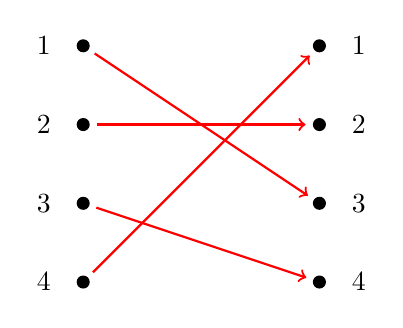
\begin{tikzpicture}
  \filldraw[black] (-1.5,0) circle (.5ex) {};
  \filldraw[black] (-1.5,1) circle (.5ex) {};
  \filldraw[black] (-1.5,2) circle (.5ex) {};
  \filldraw[black] (-1.5,3) circle (.5ex) {};
  \node at (-2, 0) {$4$};
  \node at (-2, 1) {$3$};
  \node at (-2, 2) {$2$};
  \node at (-2, 3) {$1$};

  \filldraw[black] (1.5,0) circle (.5ex) {};
  \filldraw[black] (1.5,1) circle (.5ex) {};
  \filldraw[black] (1.5,2) circle (.5ex) {};
  \filldraw[black] (1.5,3) circle (.5ex) {};
  \node at (2, 0) {$4$};
  \node at (2, 1) {$3$};
  \node at (2, 2) {$2$};
  \node at (2, 3) {$1$};

  \draw[thick,red,->,shorten <=5pt,shorten >=5pt] (-1.5, 3) -- (1.5, 1);
  \draw[thick,red,->,shorten <=5pt,shorten >=5pt] (-1.5, 2) -- (1.5, 2);
  \draw[thick,red,->,shorten <=5pt,shorten >=5pt] (-1.5, 1) -- (1.5, 0);
  \draw[thick,red,->,shorten <=5pt,shorten >=5pt] (-1.5, 0) -- (1.5, 3);
 \end{tikzpicture}
 \label{fig:permutace-jako-sipky}
 \caption{Permutace $\clr{\sigma}$ zakreslená šipkami.}
\end{figure}

Ačkoli je způsob zápisu do řádku intuitivní a podporuje představu permutace jako
\uv{proházení} prvků na množině, mnohem více se používá tzv. zápis v cyklech.
Důvody jsou primárně formální; z cyklického zápisu se velmi snadno totiž pozná
jak \uv{řád} permutace, tak její rozložení na \uv{transpozi\-ce}. Oba pojmy
definujeme a vysvětlíme později.

Jelikož permutace jsou bijekce z množiny do téže množiny, můžeme vždy začít v
nějakém libovolné prvku a pokračovat po šipkách, dokud se nedostaneme opět na
ten samý prvek. Tento přístup formalizuje právě zápis do cyklů. Například
zápis permutace $\clr{\sigma} = (3\;2\;4\;1)$ do cyklů by vypadal takto:
\begin{figure}[h]
 \centering
 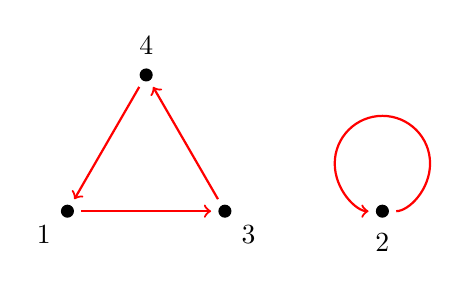
\begin{tikzpicture}
  \filldraw[black] (-1,0) circle (.5ex) {};
  \filldraw[black] (1,0) circle (.5ex) {};
  \filldraw[black] (0,1.73) circle (.5ex) {};

  \node at (-1.3, -0.3) {$1$};
  \node at (1.3, -0.3) {$3$};
  \node at (0, 2.1) {$4$};

  \filldraw[black] (3,0) circle (.5ex) {};
  \node at (3, -0.4) {$2$};

  \draw[thick,red,->,shorten <=5pt,shorten >=5pt] (-1, 0) -- (1, 0);
  \draw[thick,red,->,shorten <=5pt,shorten >=5pt] (1, 0) -- (0, 1.73);
  \draw[thick,red,->,shorten <=5pt,shorten >=5pt] (0, 1.73) -- (-1, 0);
  \draw[thick,red,->,shorten <=5pt,shorten >=5pt] (3, 0) arc (-90:270:4ex);
 \end{tikzpicture}
 \label{fig:permutace-jako-cyklus}
 \caption{Zápis permutace $\clr{\sigma}$ do cyklů.}
\end{figure}

Jak si asi dovedete představit, tento zápis znamená, že permutace $\clr{\sigma}$
pošle $1$ na $3$, pak $3$ na $4$ a nakonec $4$ na $1$. Tedy, po třech
\uv{iteracích} permutace $\clr{\sigma}$ se dostaneme z prvku $1$ opět do prvku
$1$. Smyčka nad $2$ samozřejmě znamená, že $2$ se zobrazuje opět na $2$.

Zápis na \hyperref[fig:permutace-jako-cyklus]{obrázku výše} je evidentně dosti
neúsporný, a v textu tudíž těžko použitelný. Obvykle se taková permutace zapíše
jako $\sigma = (134)(2)$. Tedy, jednotlivé cykly jsou odděleny závorkami a šipky
v cyklech vedou zleva doprava, případně z posledního prvku zpět na první.

Konečně, smyčky (tj. zobrazení prvku na sebe sama) se z cyklického zápisu běžně
vynechávají. Svoji oblíbenou permutaci $\sigma = (134)(2)$ můžeme proto úplně
nejúsporněji zapsat jako $\sigma = (134)$. Zápis permutací v cyklech budeme
odteď využívat výhradně.

\begin{warning}
 Zápis permutace pomocí cyklů \textbf{není jednoznačný}. Je to pro to, že u
 daného cyklu nelze říct, kde \uv{končí} a kde \uv{začíná}. Důležité je pouze
 vzájemné pořadí prvků. Permutace $(134), (341)$ a $(413)$ jsou tudíž jedna a ta
 samá.
\end{warning}

\subsubsection{Skládání permutací}
\label{sssec:skladani-permutaci}

Jelikož permutace jsou speciálně zobrazení, dají se pochopitelně skládat. Navíc,
protože doména i kodoména každé permutace na $X$ je právě množina $X$, mohu je
skládat v libovolném pořadí a libovolném množství.

Na výpočet složení dvou permutací $\sigma,\tau \in S_X$ není myslím žádný
vyloženě snadný postup. Člověk se musí zkrátka v cyklickém zápisu dočíst, kam
posílá první permutace daný prvek a kam zase druhá permutace posílá obraz
tohoto prvku.

\begin{example}
 Ať $X = \{1,2,3,4\}$ a $\sigma,\tau \in S_X, \sigma = (134), \tau = (14)(23)$.
 Pak
 \[
  \sigma\tau = (243),
 \]
 protože $\tau$ pošle $1$ na $4$ a $\sigma$ pošle $4$ na $1$, tedy  $\sigma\tau$
 pošle $1$ na $1$. Podobně pro ostatní prvky. V šipkách složení $\sigma\tau$ 
 vypadá takto:
 \begin{figure}[H]
  \centering
  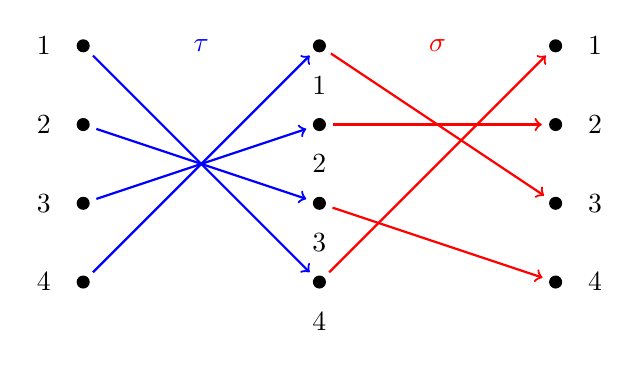
\begin{tikzpicture}
   \filldraw[black] (-1.5,0) circle (.5ex) {};
   \filldraw[black] (-1.5,1) circle (.5ex) {};
   \filldraw[black] (-1.5,2) circle (.5ex) {};
   \filldraw[black] (-1.5,3) circle (.5ex) {};
   \node at (-2, 0) {$4$};
   \node at (-2, 1) {$3$};
   \node at (-2, 2) {$2$};
   \node at (-2, 3) {$1$};

   \filldraw[black] (1.5,0) circle (.5ex) {};
   \filldraw[black] (1.5,1) circle (.5ex) {};
   \filldraw[black] (1.5,2) circle (.5ex) {};
   \filldraw[black] (1.5,3) circle (.5ex) {};
   \node at (1.5, -0.5) {$4$};
   \node at (1.5, 0.5) {$3$};
   \node at (1.5, 1.5) {$2$};
   \node at (1.5, 2.5) {$1$};

   \filldraw[black] (4.5,0) circle (.5ex) {};
   \filldraw[black] (4.5,1) circle (.5ex) {};
   \filldraw[black] (4.5,2) circle (.5ex) {};
   \filldraw[black] (4.5,3) circle (.5ex) {};
   \node at (5, 0) {$4$};
   \node at (5, 1) {$3$};
   \node at (5, 2) {$2$};
   \node at (5, 3) {$1$};

   \draw[thick,red,->,shorten <=5pt,shorten >=5pt] (1.5, 3) -- (4.5, 1);
   \draw[thick,red,->,shorten <=5pt,shorten >=5pt] (1.5, 1) -- (4.5, 0);
   \draw[thick,red,->,shorten <=5pt,shorten >=5pt] (1.5, 0) -- (4.5, 3);
   \draw[thick,red,->,shorten <=5pt,shorten >=5pt] (1.5, 2) -- (4.5, 2);

   \draw[thick,blue,->,shorten <=5pt,shorten >=5pt] (-1.5, 3) -- (1.5, 0);
   \draw[thick,blue,->,shorten <=5pt,shorten >=5pt] (-1.5, 0) -- (1.5, 3);
   \draw[thick,blue,->,shorten <=5pt,shorten >=5pt] (-1.5, 2) -- (1.5, 1);
   \draw[thick,blue,->,shorten <=5pt,shorten >=5pt] (-1.5, 1) -- (1.5, 2);

   \node[red] at (3, 3) {$\sigma$};
   \node[blue] at (0, 3) {$\tau$};
  \end{tikzpicture}
  \label{fig:slozeni-permutaci-sipky}
  \caption{Složení permutací $\clr{\sigma}\clb{\tau}$ znázorněno v šipkách.}
 \end{figure}
 Všimněte si ale, že
 \[
  \tau\sigma = (123).
 \]
\end{example}
\begin{warning}
 Jak bylo vidno z předchozího příkladu, skládání permutací (jako obecně i
 relací) \textbf{není komutativní}. Dokonce platí, že pouze skládání permutace
 se sebou samou je komutativní, čili jsou-li $\sigma,\tau \in S_X$, pak
 \[
  \sigma\tau = \tau\sigma \implies \tau = \sigma
 \]
 za předpokladu, že $\# X \geq 3$.
\end{warning}

Nyní si konečně povíme, co znamená \uv{řád} permutace a že každou permutaci lze
rozložit na \uv{transpozice}.

Když $\sigma = c_1c_2\cdots c_n$ je rozklad permutace $\sigma \in S_X$ na cykly
$c_1,c_2,\ldots,c_n$, pak \emph{délkou cyklu} $c_i$ myslíme počet prvků množiny
$X$, které se v něm vyskytují. Tedy, např. délka cyklu $(1324)$ je $4$ a délka
cyklu $(457)$ je $3$.

\begin{definition}[Transpozice]
\label{def:transpozice}
 Permutace $\sigma \in S_X$ se nazývá \emph{transpozice}, když obsahuje právě
 jeden cyklus délky $2$. Lidsky řečeno, transpozice jsou přesně ty permutace,
 které prohazují dva prvky.
\end{definition}

Možná trochu překvapivý výsledek ohledně permutací je, že každou permutaci lze
napsat jako složení transpozic. Navíc je algoritmus velmi přímočarý -- stačí
zkrátka každý cyklus délky $k$ rozložit na $k - 1$ transpozic tak, že každý
\uv{vnitřní} prvek cyklu zdvojíme. Zformulujeme si tvrzení a ukážeme si
algoritmus na příkladě.

\begin{claim}[Rozklad na transpozice]
 Ať $\sigma \in S_X$ a $\# X \geq 2$ (jinak bychom neměli dva prvky k
 prohození). Pak existují transpozice $\tau_1,\ldots,\tau_n$ takové, že
 \[
  \sigma = \tau_1\tau_2\cdots \tau_n.
 \]
 Navíc, počet transpozic v rozkladu $\sigma$ je určen jednoznačně.
\end{claim}
\begin{proof}
 Formální. Vynechám. Ideu si ukážeme na příkladě.
\end{proof}

\begin{example}
 Rozložíme permutaci $\sigma = (1342)(576)$ na transpozice. Každý cyklus vlastně
 rozdělíme na cykly délky dva (což jsou vlastně transpozice) zdvojením každého
 vnitřního prvku. Tedy, cyklus $(576)$ se rozdělí na transpozice $(57)$ a $(76)$
 a cyklus  $(1342)$ se rozdělí na $(13)$, $(34)$ a $(42)$. Pak dostaneme
 (\textbf{pozor na pořadí!})
 \[
  \sigma = (13) \circ (34) \circ (42) \circ (57) \circ (76),
 \]
 což je rozklad $\sigma$ na transpozice. Na
 \hyperref[fig:rozklad-na-transpozice]{obrázku} vidíte znázornění aplikace
 permutace $\sigma$ na množinu $\{1,\ldots,7\}$ a postupnou aplikaci příslušných
 transpozic.
 \begin{figure}[H]
  \centering
  \begin{tikzcd}
   1 \; 2 \; 3 \; 4 \; 5 \; 6 \; 7 \ar[ddddd, "\sigma = (1342)(576)"'] & 1 \; 2 \; 3 \; 4 \; 5 \; 6 \; 7 \arrow[d, "(76)"] \\
   & 1 \; 2 \; 3 \; 4 \; 5 \; 7 \; 6 \arrow[d, "(57)"] \\
   & 1 \; 2 \; 3 \; 4 \; 7 \; 5 \; 6 \ar[d, "(42)"] \\
   & 1 \; 4 \; 3 \; 2 \; 7 \; 5 \; 6 \ar[d, "(34)"] \\
   & 1 \; 3 \; 4 \; 2 \; 7 \; 5 \; 6 \ar[d, "(13)"] \\
   3 \; 1 \; 4 \; 2 \; 7 \; 5 \; 6 & 3 \; 1 \; 4 \; 2 \; 7 \; 5 \; 6
  \end{tikzcd}
  \label{fig:rozklad-na-transpozice}
  \caption{Znázornění rozkladu permutace $\sigma$ na transpozice.}
 \end{figure}
\end{example}

\begin{definition}[Sudá/lichá permutace]
\label{def:suda/licha-permutace}
 Permutaci $\sigma \in S_X$ nazveme \emph{sudou}, když její rozklad na
 transpozice obsahuje sudý počet transpozic. Jinak ji nazveme \emph{lichou}.
\end{definition}

Poslední zajímavý výsledek o permutacích, který zmíníme, říká, že když jednu
permutaci složím samu se sebou dostatečněkrát, dostanu identické zobrazení na
$X$. Počtu složení se formálně říká \uv{řád} permutace.

\begin{definition}[Řád permutace]
\label{def:rad-permutace}
 Mějme $\sigma \in S_X$. Přirozené nenulové číslo ${k \in \N}$ nazveme
 \emph{řádem} permutace $\sigma$, když
 \[
  \sigma^{k} = \mathds{1}_X,
 \]
 kde výrazem $\sigma^{k}$ myslíme složení $\sigma$ se sebou samou $k$-krát, tj.
 \[
  \sigma^{k} \coloneqq \underbrace{\sigma \circ \sigma \circ \cdots \circ
  \sigma.}_{k\text{-krát}}
 \]
 Řád permutace $\sigma$ značíme $\ord \sigma$ (z angl. \textbf{ord}er).
\end{definition}

Na konec podsekce si rozmyslíme, že každá permutace má konečný řád a jak ho
počítat. Uvažme třeba permutaci $\sigma = (143)$. Tahle permutace posílá $1$ na
$4$, $4$ na $3$ a $3$ zpět na $1$. To ovšem znamená, že když ji \uv{zopakuji}
třikrát za sebou, dostanu se rovnou z $1$ na $1$. Vskutku, můžete si ověřit, že
\[
 \sigma^3 = (143) \circ (143) \circ (143) = \mathds{1}_{\{1,2,3,4\}}.
\]
Tento pohled napovídá, že když cyklus délky $k$ zopakuji $k$-krát, zobrazím
všechny prvky v tomto cyklu na ony samé.

Co když mám ale permutaci složenou z cyklů různých délek, jako třeba
$(143)(25)$? No, cyklus $(143)$ musím zopakovat třikrát a cyklus $(25)$ dvakrát.
Když ale tuto permutaci třikrát zopakuji, nedostanu identické zobrazení, protože
cyklus $(25)$ zopakovaný třikrát je zase $(25)$. Když se zamyslíme, zjistíme, že
abych dostal z permutace identické zobrazení, musím ji opakovat právě tolikrát,
kolik je nejmenší společný násobek délek jejích cyklů, aby se každý cyklus
zopakoval nějakým násobkem své délky. Zformulujeme si tento fakt jako tvrzení,
ale dokazovat ho nebudeme, protože důkaz je otravně formální a ideu jsme si
právě řekli.

\begin{claim}[O řádu permutace]
 Ať $\sigma \in S_X$ a
 \[
  \sigma = c_1c_2\cdots c_n
 \]
 je zápis $\sigma$ v cyklech $c_1,\ldots,c_n$. Označme $d_i$ délku cyklu $c_i$ 
 pro každé $i \leq n$. Pak
 \[
  \ord \sigma = \mathrm{lcm}(d_1,\ldots,d_n),
 \]
 kde $\mathrm{lcm}$ (z angl. \textbf{l}east \textbf{c}ommon \textbf{m}ultiple)
 značí nejmenší společný násobek.
\end{claim}

Myslím, že tohle tvrzení je pěkným příkladem přirozeného avšak poměrně silného
tvrzení. Kdybyste nevěděli nic o permutacích a řekl bych vám, že máte dokázat
fakt, že když bijekci na konečné množině složím samu se sebou hodněkrát, dostanu
identické zobrazení, asi byste se zapotili.

\subsubsection{Problém sta vězňů}
\label{sssec:problem-sta-veznu}

Za sedmero horami a sedmero řekami, byla nebyla kdysi jedna věznice, ve které
bylo žilo a živořilo sto vězňů. Její dozorce, chor a zchřadl, matematik řemeslem
a krutovládce povahou, jednoho jitra rozhodl, že vězně propustí -- buď do světa,
nebo až do toho příštího.

Vyklidiv vězeňskou jídelnu, postavil zde sto dřevěných stolic nesoucích sto
papírových obálek. Mezi obálky rozloučil sto kamení, v každém toporně vyryto
různé číslo od jedné do sta.

Rozkázav vězně seřaditi před jídelnu, přičlenil každému rovněž různé číslo od
jedné do sta, v pořadí, kterak stáli. Vězni měli po řadě postoupit do jídelny a
otevřít padesát obálek. Našli-liž mezi nimi kámen zračící jejich číslo, vrátili
jej zpět a směli opustit jídelnu opačným východem.

Podmínka propuštění děla, že každý vězeň musí v jedné z padesáti obálek, které
otevřel, uzřít své číslo. Pokud byť i jeden vězeň své číslo neobjevil, celé
těleso vězňů bylo by kvapně popraveno.

Asi není těžké si rozmyslet, že tohle je úloha na permutace. Pořadí, v~jakém
jsou umístěny stolice, můžeme vnímat jako množinu přirozených čísel
$\{1,\ldots,100\}$ a rozmístění kamenů do obálek jako jednu její náhodně
zvolenou permutaci. Tedy to, že v obálce číslo $6$ je kámen s číslem $23$,
znamená, že tato permutace posílá prvek $6$ na prvek $23$.

Pokud by vězni vybírali obálky k otevření náhodně, měl by každý z nich na
nalezení kamene se svým číslem šanci přesně $1 / 2$. Protože tahle situace se má
opakovat stokrát po sobě, šance, že všichni najdou tímto způsobem své číslo, je
$(1 / 2)^{100}$, tedy $1$ ku $1 267 650 600 228 229 401 496 703 205 376$ -- čili
pořád větší, než že si MŠMT všimne, že existují počítače -- ale přesto malá.

My tvrdíme, že ve skutečnosti existuje strategie, která umožní vězňům uniknout
poslednímu dechu s šancí větší než 30 \%. Navíc je velmi přímočará. Stačí, aby
každý vězeň otevíral obálky v pořadí, které určují kameny v nich obsažené.
Konkrétně, každý vězeň otevře jako první obálku na stolici se stejným pořadím,
jako je to jeho. Dál půjde otevřít obálku na stolici s~pořadím, které odpovídá
číslu na kameni v obálce, kterou právě otevřel. Takhle pokračuje, dokud nenajde
své číslo, nebo dokud neprojde padesát různých obálek.

Ilustrujme si postup na příkladě. Do jídelny vstoupí vězeň s číslem $11$. Otevře
obálku číslo $11$ a najde v ní kámen s číslem $34$. Dále otevře obálku s číslem
$34$, v níž je číslo $77$. Ještě jednou, v obálce číslo $77$ najde číslo $5$.
V~obálce číslo $5$ najde kámen s číslem $97$. A nakonec -- Ejhle! -- v obálce
číslo $97$ najde kámen se svým číslem -- $11$.

Označme permutaci určenou čísly na kamenech v obálkách třeba $\kappa$ (podle
slova \textbf{k}ámen). Situace v předchozím odstavci znamená, že v $\kappa$
existuje cyklus
\begin{center}
 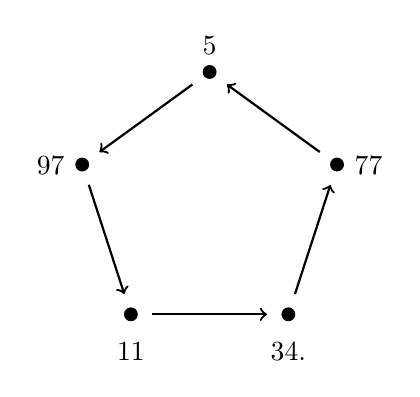
\begin{tikzpicture}
  \node[circle,fill=black,inner sep=0pt,minimum
  size=5pt,label={[yshift=-0.8cm]$11$}] (a) at (0,0) {};
  \path (a) ++(0:2) node [circle,fill=black,inner sep=0pt,minimum
  size=5pt,label={[yshift=-0.8cm]$34$.}] (b) {};
  \path (b) ++(72:2) node [circle,fill=black,inner sep=0pt,minimum
  size=5pt,label={[shift={(0.4cm, -0.35cm)}]$77$}] (c) {};
  \path (c) ++(144:2) node [circle,fill=black,inner sep=0pt,minimum
  size=5pt,label={[shift={(0cm, 0cm)}]$5$}] (d) {};
  \path (d) ++(216:2) node [circle,fill=black,inner sep=0pt,minimum
  size=5pt,label={[shift={(-0.4cm, -0.35cm)}]$97$}] (e) {};

  \draw[thick,->,shorten <=5pt,shorten >=5pt] (a) -- (b);
  \draw[thick,->,shorten <=5pt,shorten >=5pt] (b) -- (c);
  \draw[thick,->,shorten <=5pt,shorten >=5pt] (c) -- (d);
  \draw[thick,->,shorten <=5pt,shorten >=5pt] (d) -- (e);
  \draw[thick,->,shorten <=5pt,shorten >=5pt] (e) -- (a);
 \end{tikzpicture}
\end{center}

Nyní už si můžeme rozmyslet, za jaké podmínky objeví všichni vězni obál\-ku s
kamenem svého čísla. V moment, kdy vězeň otevře první obálku, dostane se tím do
jednoho konkrétního cyklu permutace $\kappa$. Podle dané strategie bude tento
cyklus sledovat až do konce (když \uv{začátkem} cyklu myslíme číslo vězně).
Pokud je délka daného cyklu třeba $d$, pak v moment, kdy otevře tento vězeň
$d$-tou obálku, bude v ní kámen s jeho číslem. Samozřejmě, podmínka propuštění
říkala, že každý vězeň smí otevřít maximálně $50$ obálek. Protože každý vězeň má
přiřazeno jiné, určitě čísla všech vězňů dohromady vyčerpají všechny cykly
permutace $\kappa$. To znamená, že všichni vězni najdou svoje číslo tímto
postupem jedině v případě, \textbf{kdy permutace $\kappa$ neobsahuje cyklus
délky větší než 50}. Zformulujeme si to jako pozorování.

\begin{observation}
 Problém sta vězňů má řešení (tedy všech sto vězňů bude propuštěno) právě tehdy,
 když permutace $\kappa$, určená čísly na kamenech v obálkách, neobsahuje cyklus
 délky větší než $50$.
\end{observation}

Abychom spočítali šanci vězňů na úspěch, zbývá nám umět spočítat počet všech
takových permutací, tj. permutací s cykly délky maximálně $50$.

Ať $X \coloneqq \{1,\ldots,100\}$. Bude výhodnější řešit opačný problém, tedy
hledat počet permutací s cyklem délky aspoň $51$, protože (vzhledem k tomu, že
množina $X$ má $100$ prvků), takový cyklus tam může být nejvýše jeden.

Ať $C_n(S_X)$ značí počet všech permutací na $X$ s aspoň jedním cyklem délky
$n$. Jak jsme právě řekli, pro $n \geq 51$ může mít libovolná permutace takový
cyklus jenom jeden. Dále je zřejmé, že počet všech permutací s cyklem délky
\emph{aspoň} $51$ spočtu tak, že sečtu počty permutací s cyklem délky $n$ pro
všechna $n$ od $51$ do $100$. Když $C_{ \geq 51}(S_X)$ značí počet permutací s
cyklem délky aspoň $51$, máme
\[
 C_{ \geq 51}(S_X) = \sum_{n=51}^{100} C_n(S_X). 
\]

Spočítáme $C_n(S_X)$ pro $n \geq 51$. Abychom určili permutace s cyklem délky
$n$, musíme zvolit $n$ z těch $100$ čísel, která se v cyklu objeví. Počet
způsobů, jak zvolit $n$ čísel ze $100$ je $\binom{100}{n}$ (vizte
\hyperref[ssec:kombinacni-cisla]{sekci o
kombinačních číslech}).
Čísla v tomto cyklu mohou být uspořádána $n!$ způsoby. \textbf{Ovšem, pozor!}
Nezapomeňte, že uvnitř cyklu mohu čísla posouvat a cyklus tím nechat stejný.
Protože mám v cyklu $n$ čísel, dělá to dohromady $n$ možných posunutí. Tedy mám
\[
 \frac{\binom{100}{n}n!}{n} = \binom{100}{n}(n-1)!
\]
různých způsobů, jak zvolit cyklus délky $n$.

Konečně, zbývající čísla (tedy ta mimo ten cyklus) můžu přeuspořádat $(100-n)!$
způsoby. Celkem, počet všech permutací s cyklem délky $n$ pro $n \geq 51$ je
\[
 C_n(S_X) = \binom{100}{n}(n-1)!(100-n)!.
\]
Je na čase završit výpočet. Všech možných permutací na $100$ číslech je $100!$.
Počet všech permutací s cyklem délky aspoň $51$ je $C_{\geq 51}(S_X)$. Čili šance,
že náhodně vybraná permutace na $100$ číslech \textbf{obsahuje} cyklus délky
větší než $50$ je
\[
 \frac{C_{ \geq 51}(S_X)}{100!} = \frac{\sum_{n=51}^{100} C_n(S_X)}{100!} =
 \frac{\sum_{n=51}^{100} \binom{100}{n}(n-1)!(100-n)!}{100!} \approx 0.688,
\]
čili $68,8~\%$. To ovšem znamená, že šance, že náhodná permutace
\textbf{neobsahuje} cyklus délky větší než $50$ je přibližně $1 - 0.688 =
0.312$. Takže při využití této strategie mají vězni přibližně $31.2\%$ šanci na
přežití. O něco lepší než náhodné zkoušení.

\begin{exercise}
 Spočtěte složení $\sigma\tau$ a $\tau\sigma$, když
 \begin{enumerate}[topsep=0pt,label=(\arabic*)]
  \item $\sigma = (143)(26), \tau = (146)(253)$,
  \item $\sigma = (14)(25)(36), \tau = (123456)$,
  \item $\sigma = (145)(263), \tau = (154)(236)$.
 \end{enumerate}
\end{exercise}

\begin{exercise}
 Určete řád permutace $\sigma$, kde
 \begin{enumerate}[label=(\arabic*),topsep=0pt]
  \item $\sigma = (1345)$,
  \item $\sigma = (1346)(28)(579)$.
 \end{enumerate}
\end{exercise}

\begin{exercise}[těžké]
 Určete číslo $C_n(S_X)$, kde $\# X = 100$ a $n \leq 50$, tedy počet všech
 permutací na $100$ číslech s aspoň jedním cyklem délky menší nebo rovné
 $50$.

 Samozřejmě jich je $100! - C_{ \geq 51}(S_X)$, ale cílem úlohy je spočítat je
 nějak chytře, aby člověk dostal hezčí vzoreček.
\end{exercise}

\begin{exercise}
 Ať $\sigma \in S_n$, tedy $\sigma$ je permutace množiny $\{1,\ldots,n\}$.
 Řekneme, že $\sigma$ \emph{invertuje} dvojici $(i,j)$, kde $i,j \in
 \{1,\ldots,n\}$, když $i<j$, ale $\sigma(i)>\sigma(j)$.

 Definujme
  \[
   I(\sigma) \coloneqq \{(i,j) \in \{1,\ldots,n\}^2 \mid \sigma \text{ invertuje
   } (i,j)\},
 \]
 čili $I(\sigma)$ je množina všech dvojic $(i,j)$, které $\sigma$ invertuje.
 Uvědomme si, že $I(\sigma)$ je podmnožinou $\{1,\ldots,n\}^2$, čili relací na
 $\{1,\ldots,n\}$.
 \begin{enumerate}[label=(\arabic*),topsep=0pt]
  \item Dokažte, že $I(\sigma)$ je transitivní relace na $\{1,\ldots,n\}$ pro
   každou permutaci $\sigma \in S_n$.
  \item* Navrhněte algoritmus, který pro danou permutaci $\sigma \in S_n$ spočte
   $\# I(\sigma)$.
  \item Spočtěte počet invertovaných dvojic, čili $\# I(\sigma)$, permutací
   $\sigma = (134)(579)(26)$.
 \end{enumerate}
\end{exercise}

\subsection{Kombinační čísla}
\label{ssec:kombinacni-cisla}

V této sekci se budeme zabývat asi poměrně přirozenou otázkou -- kolik má
množina $X$ podmnožin velikosti $k$, kde $k$ může být libovolné číslo od $0$ do
$\# X$. Pro $k=0$ i $k=\# X$ je odpověď jednoduchá: přesně jednu. Pro $k = 1$
člověku hádám taky dojde, že jednoprvková podmnožina je vlastně totéž, co její
jediný prvek, takže takových máme $\# X$. Od $k = 2$ nám ale začína, borcovia,
prituhovať. Nejspíš bychom pořád zvládli počet dvouprvkových množin nějak
zpatlat, ale co třeba $k = \# X / 2$ (když je $\# X$ sudé) a podobné takřka
nekřesťanské výmysly? To už chce nějaké udělátko.

Nejdřív si to ale, jakožto slušní a spořádaní matematikové, definujeme.

\begin{definition}[Počet $k$-prvkových podmnožin]
 Ať $X$ je množina a $0 \leq k \leq \# X$ je přirozené číslo. Definujeme množinu
 \[
  \binom{X}{k} \coloneqq \{A \subseteq X \mid \# A = k\}
 \]
 všech $k$-prvkových podmnožin množiny $X$. Výraz $\binom{X}{k}$ čteme \uv{$X$ 
 nad $k$}.
\end{definition}

Chvilku se budeme bavit přemítáním o způsobu, jak spočítat $\# \binom{X}{k}$ pro
libovolné $k$ mezi $0$ a $\# X$.

Použijeme kombinatorickou metodu důkazu zvanou \emph{počítání dvěma způsoby}.
Jde o užitečný (a podle mého velmi elegantní) přístup ve chvíli, kdy neumím
spočítat rovnou konkrétní množství, ale umím spočítat něco vel\-mi podobného.
Technika počítání dvěma způsoby spočívá v tom, že tu kvantitu, kterou spočítat
\emph{umím}, vyjádřím na jedné straně pomocí kvantity, kterou spočítat
\emph{neumím}, a na druhé straně pomocí vzorečku, který znám. To mi dá rovnici,
ze které pak vyjádřím to číslo, které chci určit.

Takto abstraktně vám asi \emph{počítání dvěma způsoby} nic neřeklo, takže je
raději pojďme aplikovat na zpytovaný problém. Počet $k$-prvkových podmnožin $X$
spočítat neumím; což takhle začít tím, že si nějakou náhodnou podmnožinu
$\{x_1,\ldots,x_k\} \subseteq X$ zvolím. Jeden z důvodů, proč neumím počet
takovýchhle podmnožin spočítat, je, že mi chybí nějaké \emph{uspořádání}.

Zatím všechny věci, které jsme počítali, byly v jistém smyslu \emph{uspořádané}.
Počet všech zobrazení $A \to B$ jsme počítali tak, že jsme prvky $A$
\textbf{jeden po druhém} zobrazovali na prvky $B$. Vlastně nevědomky jsme si tak
nějakým náhodným způsobem \emph{uspořádali} množinu $A$, aby se nám dobře
počítalo. Permutace jsou taky přímo definované tak, že mění \emph{uspořádání}
prvků na množině.

Vybrat si nějaké uspořádání na $X$ a všechny její podmnožiny pak považovat za
uspořádané podle stejného uspořádání je chytrý nápad, který přinese ovoce. Na
konci výpočtu je však potřeba zanedbat všechny možné způsoby, kterými jsme 
$k$-prvkové množiny mohli uspořádat. Uvidíte, že nám nakonec opravdu vyjde, že
počet všech $k$-prvkových podmnožin $X$ je vlastně počet všech $k$-prvkových
podmnožin $X$ s nějakým konkrétním uspořádáním dělen počtem způsobů, kolika jsme
takové uspořádání mohli zvolit.

Pojďme tedy místo množiny $\{x_1,\ldots,x_k\}$ uvažovat její \uv{uspořádanou
verzi}, tím míním $k$-tici $(x_1,\ldots,x_k)$. Rozdíl je samozřejmě v tom, že
(třeba pro $k = 3$) je množina $\{x_1,x_2,x_3\}$ ta samá, co $\{x_2,x_1,x_3\}$,
ale trojice $(x_1,x_2,x_3)$ je různá od trojice $(x_2,x_1,x_3)$. Záleží na
pořadí, v jakém prvky za sebe umisťuji, na \emph{uspořádání}.

Na první straně rovnice vzniklé \emph{počítáním dvěma způsoby} si určíme, kolik
různých takových $k$-tic mi z jedné množiny může vzniknout. No přeci tolik,
kolika způsoby mohu mezi sebou proházet (nebo třeba cizeji \uv{pro\-permutovat}
$\leftarrow$ hint btw) její prvky. Každá permutace na $\{x_1,\ldots,x_k\}$ mi
určuje přesně jedno možné uspořádání. Těch je, podle
\hyperref[prop:pocet-permutaci-na-mnozine]{tvrzení~\ref*{prop:pocet-permutaci-na-mnozine}},
$k!$. Z~definice máme $\# \binom{X}{k}$ různých $k$-prvkových podmnožin $X$ a
každá určuje $k!$ uspořádaných $k$-tic. Celkem těchto tedy máme $k! \cdot \#
\binom{X}{k}$. To činí jednu stranu naší rovnice.

Na druhé straně, vybrat $k$ prvků z $X$ a nějak je uspořádat je přeci to samé,
jako jim nějak přiřadit čísla od $1$ do $k$. Takovéhle přiřazení mi určí přesně,
v jakém pořadí prvky $x_1,\ldots,x_k$ jsou. Tedy, ten prvek, který dostane $1$,
jde první, ten s $2$ jde druhý atd.

Uvědomme si, že výběr přesně $k$ prvků z množiny $X$ a jejich následné
uspořádání (tedy přiřazení čísel od $1$ do $k$) je vlastně prosté zobrazení ${f:
\{1,\ldots,k\} \to X}$. Každému takovému zobrazení odpovídá uspořádaná $k$-tice
$(f(1),\ldots,f(k))$ prvků z $X$ a naopak každou $k$-tici $(x_1,\ldots,x_k)$
lze považovat za prosté zobrazení $g: \{1,\ldots,k\} \to X$ takové, že
$g(i)=x_i$ pro všechna $i \leq k$. Čili, pro každou podmnožinu
$\{x_1,\ldots,x_k\} \subseteq X$ mám tolik uspořádaných $k$-tic
$(x_1,\ldots,x_k)$ jako mám prostých zobrazení $\{1,\ldots,k\} \to X$. Podle
\hyperref[claim:pocet-prostych-zobrazeni]{tvrzení~\ref*{claim:pocet-prostych-zobrazeni}}
je tento počet roven $\prod_{i=0}^{k-1} \#X-i$.

Na závěr již stačí obě množství vzniklá dvěma různými způsoby počítání
uspořádaných $k$-prvkových podmnožin $X$ porovnat. Dostaneme
\[
 \prod_{i=0}^{k-1} \# X-i = k! \cdot \# \binom{X}{k}, 
\]
odkud okamžitě plyne
\[
 \# \binom{X}{k} = \frac{\prod_{i=0}^{k-1} \# X - i}{k!}.
\]

Diskuse tvořící obsah předchozích dvou stránek je velmi obšírným důkazem
následujícího tvrzení.

\begin{claim}[Počet $k$-prvkových podmnožin]
 \label{claim:pocet-k-prvkovych-podmnozin}
 Ať $X$ je konečná množina. Pak počet všech $k$-prvkových podmnožin $X$ je roven
 \[
  \frac{\prod_{i=0}^{k-1} \# X - i}{k!}.
 \]
\end{claim}

K tomuto tvrzení se víže definice tzv. \emph{kombinačního čísla}.

\begin{definition}[Kombinační číslo]
 \label{def:kombinacni-cislo}
 Ať $k,n \in \N$ a $k \leq n$. Pak definujeme
 \[
  \binom{n}{k} \coloneqq \frac{\prod_{i=0}^{k-1} n-i }{k!}.
 \]
 Výraz $\binom{n}{k}$ čteme $n$ nad $k$.
\end{definition}

V závěsu \hyperref[def:kombinacni-cislo]{definice~\ref*{def:kombinacni-cislo}}
můžeme
\hyperref[claim:pocet-k-prvkovych-podmnozin]{tvrzení~\ref*{claim:pocet-k-prvkovych-podmnozin}}
přepsat jako rovnost
\[
 \# \binom{X}{k} = \binom{\# X}{k}.
\]

Ve škole se často učí interpretace kombinačního čísla $\binom{n}{k}$ jako
\uv{počet způsobů, jak volit $k$ předmětů z $n$ bez závislosti na pořadí}. Ta je
plně v souladu s naší definicí, interpretujeme-li $X$ jako množinu předmětů a
jednu její $k$-prvkovou podmnožinu jako výběr $k$ předmětů, kde však
pochopitelně (jedná se o \textbf{podmnožinu}) nezáleží na jejich uspořádání.

\subsubsection{Problém rozkladu na sčítance}
\label{sssec:problem-rozkladu-na-scitance}

Oblíbený problém, který lze řešit počítáním způsobů, jak volit počet sourodých
předmětů z většího množství, ale nikdo by to na první pohled nečekal, je
\emph{problém rozkladu na sčítance}.

Volme číslo $m \in \N$. \emph{Rozkladem čísla $m$ na $r$ sčítanců} myslíme
rovnost
\[
 m = x_1 + x_2 + \cdots + x_r = \sum_{k=1}^{r} x_k,
\]
kde $x_i \geq 0$ jsou nezáporná celá čísla. Zajímá nás, kolika způsoby lze dané
číslo $m$ rozložit na $r$ (ne nutně různých) sčítanců. Na první pohled nejde
vůbec o kombinace (tedy o výběr bez závislosti na pořadí), protože pořadí
sčítanců je zde důležité: rozklad $7 = 0 + 2 + 5$ \textbf{je různý} od rozkladu
$7 = 2 + 0 + 5$. Situace se navíc v tomto směru zdá zcela beznadějná, neboť když
jsou dvě a více čísel v rozkladu stejná, pak jejich prohození samozřejmě
neurčuje jiný rozklad. Například, v rozkladu $7 = 2 + 2 + 3$ mohu prohodit první
$2$ s druhou $2$ a nedostat tak odlišný rozklad.

První průlomovou myšlenkou je náhled, že číslo $m$ vlastně \uv{rozhazuji} mezi
$r$ čísel. V tomto smyslu si lze představit přirozené číslo $m$ jako $m$
nerozlišitelných míčků, které rozděluji do $r$ košíků. Třeba rozklad $7 = 0 + 2
+ 5$ by vypadal takto.

\begin{figure}[h]
 \centering
 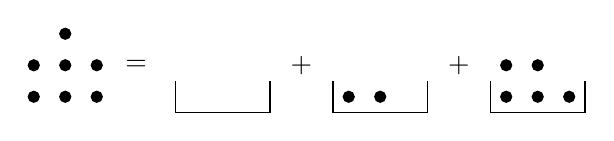
\begin{tikzpicture}
  \foreach \i in {-0.4,0} {
   \foreach \j in {0,0.4,0.8} {
    \draw[fill=black]  (\j, \i) circle (2pt);
   }
  }
  \draw[fill=black] (0.4, 0.4) circle (2pt);

  \node at (1.3, 0) {$=$};

  \foreach \j in {0,0.4} {
   \draw[fill=black]  (4 + \j, -0.4) circle (2pt);
  }

  \draw (1.8, -0.2) -- (1.8,-0.6);
  \draw (1.8, -0.6) -- (3,-0.6);
  \draw (3, -0.6) -- (3,-0.2);

  \node at (3.4,0) {$+$};

  \draw (3.8, -0.2) -- (3.8,-0.6);
  \draw (3.8, -0.6) -- (5,-0.6);
  \draw (5, -0.6) -- (5,-0.2);

  \node at (5.4,0) {$+$};

  \foreach \j in {0,0.4,0.8} {
   \draw[fill=black]  (6 + \j, -0.4) circle (2pt);
  }
  \draw[fill=black]  (6, 0) circle (2pt);
  \draw[fill=black]  (6.4, 0) circle (2pt);

  \draw (5.8, -0.2) -- (5.8,-0.6);
  \draw (5.8, -0.6) -- (7,-0.6);
  \draw (7, -0.6) -- (7,-0.2);
 \end{tikzpicture}
 \label{fig:micky-do-kosiku}
 \caption{Vizualizace rozkladu $7 = 0 + 2 + 5$ jako rozdělení míčků do košíků.}
\end{figure}

Samozřejmě, v takovémto rozkladu určuje pravá strana jednoznačně tu levou, takže
není třeba $7$ míčků na levé straně znázorňovat. Podobně, když se dohodneme, že
počty míčků v košících vždy sčítáme, lze i symboly $+$ vynechat. Trochu
složitější rozklad, třeba $9 = 1 + 0 + 3 + 5$ bychom nakreslili jak vidno na
\hyperref[fig:jenom-micky-a-kosiky]{obrázku~\ref*{fig:jenom-micky-a-kosiky}}.

\begin{figure}[h]
 \centering
 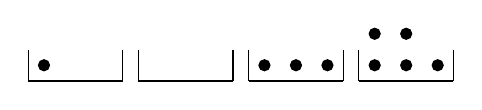
\begin{tikzpicture}
  \foreach \k in {0} {
   \draw (\k,-0.2) -- (\k,-0.6);
   \draw (\k,-0.6) -- (\k+1.2,-0.6);
   \draw (\k+1.2,-0.6) -- (\k+1.2,-0.2);
  }
  \draw[fill=black]  (0.2, -0.4) circle (2pt);

  \foreach \k in {1.4} {
   \draw (\k,-0.2) -- (\k,-0.6);
   \draw (\k,-0.6) -- (\k+1.2,-0.6);
   \draw (\k+1.2,-0.6) -- (\k+1.2,-0.2);
  }

  \foreach \k in {2.8} {
   \draw (\k,-0.2) -- (\k,-0.6);
   \draw (\k,-0.6) -- (\k+1.2,-0.6);
   \draw (\k+1.2,-0.6) -- (\k+1.2,-0.2);
  }
  \foreach \j in {0,0.4,0.8} {
   \draw[fill=black]  (3 + \j, -0.4) circle (2pt);
  }

  \foreach \k in {4.2} {
   \draw (\k,-0.2) -- (\k,-0.6);
   \draw (\k,-0.6) -- (\k+1.2,-0.6);
   \draw (\k+1.2,-0.6) -- (\k+1.2,-0.2);
  }
  \foreach \j in {0,0.4,0.8} {
   \draw[fill=black]  (4.4 + \j, -0.4) circle (2pt);
  }
  \foreach \j in {0,0.4} {
   \draw[fill=black]  (4.4 + \j, 0) circle (2pt);
  }
 \end{tikzpicture}
 \caption{Zjednodušený nákres rozdělení míčků do košíků.}
 \label{fig:jenom-micky-a-kosiky}
\end{figure}

Nakonec si uvědomíme, že přeci není ani třeba kreslit jednotlivé košíky. Stačí,
když všechny míčky vysypeme na zem a jenom mezi ně dáme nějaká hradla, abychom
věděli, které míčky patřily do stejného košíku. Názorná ukázka, pro stejný
rozklad, tedy $9 = 1 + 0 + 3 + 5$.

\begin{figure}[h]
 \centering
 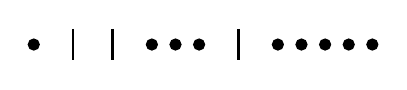
\begin{tikzpicture}
  \draw[fill=black] (0, 0) circle (2pt);
  \draw[thick] (0.5, 0.2) -- (0.5, -0.2);
  \draw[thick] (1, 0.2) -- (1, -0.2);
  
  \foreach \i in {0,0.3,0.6} {
   \draw[fill=black] (1.5 + \i, 0) circle (2pt);
  }

  \draw[thick] (2.6, 0.2) -- (2.6, -0.2);
  \foreach \i in {0,0.3,...,1.5} {
   \draw[fill=black] (3.1 + \i, 0) circle (2pt);
  }
 \end{tikzpicture}
 \caption{Ještě jednodušší nákres rozkladu $9 = 1 + 0 + 3 + 5$.}
 \label{fig:nejjednodussi-micky-s-kosiky}
\end{figure}

Jeden možný způsob, jak si snadno představit spojitost mezi rozkladem a touto
poslední verzí jeho vizualizace je ten, že stěny či hradla odpovídají symbolům
$+$ a počet míčku mezi dvěma hradly odpovídá číslu mezi příslušnými symboly.
Protože sčítanců je $r$, a tedy symbolů $+$ je $r - 1$, je hradel též $r - 1$.

Jsme připraveni řešení úlohy završit. Rozmysleli jsme si, že každé rozmístění $r
- 1$ hradel mezi $m$ za sebou v řadě ležících míčků mi definuje jeden konkrétní
rozklad čísla $m$ na $r$ sčítanců. Stačí tedy umět určit počet takových
rozmístění.

To ale není těžké. Míčky a hradla činí dohromady $m + r - 1$ objektů, z kterých
přesně $r - 1$ jsou hradla. Řečeno jinak, když z $m + r - 1$ objektů vyberu těch
$r - 1$, která se stanou hradly, a zbytek přetvořím v míčky, pak určím rozklad
čísla $m$ na $r$ sčítanců. Počet všech možných výběrů $r - 1$ prvků z~množiny o
$m + r - 1$ prvcích je $\binom{m + r - 1}{r-1}$, kteréžto číslo je tudíž i počet
způsobů, jak rozložit číslo $m$ na $r$ sčítanců.

\subsubsection{Pár vlastností kombinačních čísel}
\label{sssec:par-vlastnosti-kombinacnich-cisel}

Tahle sekce si neklade za cíl objevit zatím neznámý kontinent ani čtenáře naučit
životu v afrických pralesích. Baže naopak, jedná se o prostou přílohu k již
známému. Kombinační čísla se objevují, kdykoli člověk počítá s~podobjekty
konečných objektů, tedy v podstatě pořád. Věnujeme chvilku času prozkoumání
způsobů, jak s nimi zacházet.

Nejprve jeden výpočetně užitečný vzoreček.

\begin{lemma}
 \label{lem:vzorec-pro-kombinacni-cislo}
 Ať $k,n \in \N$, $k \leq n$. Platí
 \[
  \binom{n}{k} = \frac{n!}{k!(n-k)!}.
 \]
\end{lemma}
\begin{proof}
 Z \hyperref[def:kombinacni-cislo]{definice kombinačního čísla} máme
 \[
  \binom{n}{k} = \frac{\prod_{i=0}^{k-1} n-i}{k!},
 \]
 stačí tedy ukázat, že
 \[
  \prod_{i=0}^{k-1} n - i = \frac{n!}{(n-k)!}.
 \]
 To je však zřejmé, neboť
 \begin{align*}
  n! &= n(n-1) \cdots (n-k+1)(n-k)(n-k-1) \cdots 1\\
  &= n(n-1)\cdots (n-k+1)(n-k)! = \left( \prod_{i=0}^{k-1} n-i \right)(n-k)!.
 \end{align*}
 Důkaz plyne z vydělení poslední rovnice číslem $(n-k)!$.
\end{proof}

Dále si povíme o tzv. \emph{Pascalově trojúhelníku}. Tím se obvykle míní
následující struktura.

\begin{figure}[h]
 \centering
 \begin{tikzpicture}
  \node at (0,0.5) {$1$};

  \node at (-0.5,0) {$1$};
  \node at (0.5,0) {$1$};

  \node at (-1,-0.5) {$1$};
  \node at (0,-0.5) {$2$};
  \node at (1,-0.5) {$1$};

  \node at (-1.5,-1) {$1$};
  \node at (-0.5,-1) {$3$};
  \node at (0.5,-1) {$3$};
  \node at (1.5,-1) {$1$};

  \node at (-2,-1.5) {$1$};
  \node at (-1,-1.5) {$4$};
  \node at (0,-1.5) {$6$};
  \node at (1,-1.5) {$4$};
  \node at (2,-1.5) {$1$};

  \node at (-2.5,-2) {$1$};
  \node at (-1.5,-2) {$5$};
  \node at (-0.5,-2) {$10$};
  \node at (0.5,-2) {$10$};
  \node at (1.5,-2) {$5$};
  \node at (2.5,-2) {$1$};

  \node at (0, -2.5) {$\vdots$};
 \end{tikzpicture}
 \caption{Pascalův trojúhelník.}
 \label{fig:pascaluv-trojuhelnik}
\end{figure}

Jde vlastně o posloupnost řad, kde na začátku a na konci každé řady je číslo $1$
a prostřední čísla dostanu tak, že sečtu ta dvě čísla z předchozí řady těsně nad
ním.

Formálně můžeme říci, že Pascalův trojúhelník je posloupnost uspořádaných
$n$-tic $(p_1^{n},\ldots,p_n^{n}) \in \N^{n}$ ($n$ jsou \textbf{indexy} řádků,
nikoli mocniny), taková, že $p_i^{n} = p_{i-1}^{n-1} + p_{i}^{n-1}$ pro každé $n
\geq 1$ a každé $1 \leq i \leq n$. Pro začátek položíme $p_1^{1} = 1$ a v každém
řádku dodefinujeme $p_{0}^{n} = p_{n+1}^{n} = 0$.

Skutečně, když $p_1^{1} = 1$, tedy první číslo prvního řádku je $1$, pak
$p_1^{2} = p_0^{1} + p_1^{1} = 0 + 1 = 1$ a $p_2^{2} = p_1^{1} + p_2^{1} = 1 + 0
= 1$, čili druhý řádek je dvojice $(1, 1)$. Zde vidíte důvod, proč jsme
dodefinovali též $0$-tý a $(n+1)$-ní prvek $n$-tého řádku. Museli bychom totiž
jinak psát speciální pravidlo pro určení prvního a posledního prvku každého
řádku. Místo toho předstíráme, že je Pascalův trojúhelník ještě z obou stran
obklopen nulami.

Pro pořádek si ještě v tomto formálním pohledu spočteme třetí řádek, tj. trojici
$(p_1^{3},p_2^{3},p_3^3)$. Máme
\begin{align*}
 p_1^3&= p_0^2+p_1^2 = 0 + 1 = 1, \\
 p_2^3&= p_1^{2}+p_2^2 = 1 + 1 = 2, \\
 p_3^3&= p_2^2 + p_3^2 = 1 + 0 = 1.
\end{align*}
Vše je, jak má být.

Budeme chtít ukázat, že $n$-tý řádek Pascalova trojúhelníku tvoří přesně čísla
$\binom{n-1}{0},\binom{n-1}{1},\ldots,\binom{n-1}{n-1}$. Pro první řádky je to
jistě pravda, neboť $\binom{0}{0} = 1$ (neboť $0!$ se tradičně definuje jako
$1$) a dále $\binom{1}{0} = \binom{1}{1} = 1$.

Rozepíšeme si, co naše tvrzení vlastně znamená z pohledu kombinačních čísel.
Prvky $p_i^{n+1}$ v $(n+1)$-ním řádku Pascalova trojúhelníku jsou definovány
pomocí prvků v předchozím řádku vzorcem $p_{i+1}^{n+1} = p_{i}^{n} +
p_{i+1}^{n}$. A my tvrdíme, že $p_{i}^{n} = \binom{n-1}{i-1}$. (Ověřte si, že to
je \textbf{opravdu} to, co říkáme!) Přepíšeme-li tuto rovnost v kombinačních
číslech, potřebujeme dokázat, že
\begin{equation*}
 \label{eq:pascal-identity}
 \tag{$*$}
 \binom{n}{i} = \binom{n-1}{i-1} + \binom{n-1}{i}
\end{equation*}
pro každé $n \geq 1$ každé $1 \leq i \leq n$.

I když by to jistě nějak šlo upočítat, my zvolíme elegantnější způsob, který
zůstává věrný tomu, co kombinační číslo vlastně \textbf{vyjadřuje}. Nezapomeňte,
že $\binom{n}{i}$ je počet $i$-prvkových podmnožin $n$-prvkové množiny. Je
jisté, že množina $(i-1)$-prvkových podmnožin je disjunktní (má prázdný průnik) s
množinou $i$-prvkových podmnožin. To ovšem znamená, že
\begin{align*}
 \# \left( \binom{\{1,\ldots,n-1\}}{i-1} \cup \binom{\{1,\ldots,n-1\}}{i}
 \right)
 &= \# \binom{\{1,\ldots,n-1\}}{i-1} + \# \binom{\{1,\ldots,n-1\}}{i}\\
 &= \binom{n-1}{i-1} + \binom{n-1}{i}.
\end{align*}
Řečeno selsky, když vezmu množinu obsahující všechny $i$-prvkové i
$(i-1)$-prvkové podmnožiny, pak její velikost je počet všech $i$-prvkových
podmnožin plus počet všech $(i-1)$-prvkových podmnožin. No shit.

Čili, abychom dokázali rovnost \eqref{eq:pascal-identity}, najdeme bijekci mezi
množinou všech $i$-prvkových a $(i-1)$-prvkových podmnožin $(n-1)$-prvkové
množiny a množinou všech  $i$-prvkových podmnožin $n$-prvkové množiny.

\begin{claim}[Pascalova rovnost]
 \label{claim:pascalova-rovnost}
 Ať $1 \leq i,n \in \N$ a $i \leq n$. Pak platí
 \[
  \binom{n}{i} = \binom{n-1}{i-1} + \binom{n-1}{i}.
 \]
\end{claim}
\begin{proof}
 Definujeme bijekci
 \[ 
  f: \binom{\{1,\ldots,n-1\}}{i-1} \cup \binom{\{1,\ldots,n-1\}}{i} \to
  \binom{\{1,\ldots,n\}}{i}.
 \]
 Ať nejprve $A \in \binom{\{1,\ldots,n-1\}}{i}$, čili $A$ je $i$-prvková
 podmnožina ${\{1,\ldots,n-1\}}$. Pak je $A$ též $i$-prvková podmnožina
 $\{1,\ldots,n\}$, neboli $A \in \binom{\{1,\ldots,n\}}{i}$ a stačí definovat
 $f(A) \coloneqq A$. Stručně řečeno, $f$ je identické zobrazení na $i$-prvkových
 podmnožinách.

 Teď ať $B \in \binom{\{1,\ldots,n-1\}}{i-1}$. Pak $B \cup \{n\}$ je $i$-prvková
 podmnožina $\{1,\ldots,n\}$ a tedy můžeme definovat $f(B) \coloneqq B \cup
 \{n\}$.

 Je zřejmé, že $f$ je bijekce. Když $A \subseteq \{1,\ldots,n\}$ neobsahuje $n$,
 pak je jejím vzorem při $f$ ta samá množina, tj. $A$. Když $A \subseteq
 \{1,\ldots,n\}$ obsahuje $n$, pak je jejím vzorem množina $A \setminus
 \{n\} \subseteq \{1,\ldots,n-1\}$.

 Tím je důkaz dokončen.
\end{proof}

\hyperref[claim:pascalova-rovnost]{Předchozí tvrzení} ukazuje, že pro $n$-tý
řádek Pascalova trojúhelníka oprav\-du platí rovnost
\[
 (p_1^{n},\ldots,p_n^{n}) = \left(
 \binom{n-1}{0},\binom{n-1}{1},\ldots,\binom{n-1}{n-1} \right).
\]

Na závěr celé sekce o kombinačních číslech si ukážeme ještě poslední snadno
dokazatelnou rovnost, která je však výpočetně též užitečná.

\begin{lemma}
 \label{lemma:stejne-doplnku}
 Ať $k,n \in \N$ a $k \leq n$. Pak
 \[
  \binom{n}{k} = \binom{n}{n-k}.
 \]
\end{lemma}
\begin{proof}
 Nalezneme bijekci
 \[
  \binom{\{1,\ldots,n\}}{k} \to \binom{\{1,\ldots,n\}}{n-k}.
 \]
 Uvědomme si, že když $A \subseteq \{1,\ldots,n\}$ a $\# A = k$, pak $\#
 (\{1,\ldots,n\} \setminus A) = n - k$. Kýžená bijekce je tudíž zobrazení $A
 \mapsto \{1,\ldots,n\} \setminus A$.
\end{proof}

Ještě několik úloh pro bystré hlavy.

\begin{exercise}
 Dokažte, že
 \[
  \sum_{i=0}^{n} \binom{n}{i}^2 = \binom{2n}{n}.
 \]
 \textbf{Hint}: použijte
 \hyperref[lemma:stejne-doplnku]{lemma~\ref*{lemma:stejne-doplnku}}.
\end{exercise}

\begin{exercise}
 Dokažte vzorec
 \[
  \sum_{k=r}^{n} \binom{k}{r} = \binom{n+1}{r+1}
 \]
 pro pevné $r \in \N$ indukcí podle $n \in \N$.
\end{exercise}

\begin{exercise}[těžké]
 Kolik existuje podmnožin $\{1,\ldots,n\}$, které neobsahují žádná dvě po sobě
 jdoucí čísla. Formálně, určete velikost množiny
 \[
  \{A \subseteq \{1,\ldots,n\} \mid \{i,j\} \nsubseteq A, \text{ kdykoli }
  |i-j|=1\}.
 \]
\end{exercise}

\begin{exercise}[trocha teorie čísel]
 Ať $p$ je prvočíslo a $k,n$ přirozená čísla.
 \begin{enumerate}[label=(\alph*),topsep=0pt]
  \item Dokažte, že pro $k<p$ je $\binom{p}{k}$ dělitelné $p$.
  \item Dokažte, že $\binom{n}{p}$ je dělitelné $p$ právě tehdy, když $\left\lfloor n
   / p \right\rfloor$ je dělitelné $p$, kde $\left\lfloor  \cdot \right\rfloor$ 
   značí \emph{dolní celou část}.
 \end{enumerate}
\end{exercise}

\begin{exercise}
 Budeme vybírat $k$-tice předmětů z $n$ druhů předmětů. Budeme uvažovat různé
 typy výběru podle toho, jestli vybíráme $k$-tice uspořádané, nebo neuspořádané
 (tj. podmnožiny) a též podle toho, zda každého druhu je vždy jen jeden předmět,
 či nikoli. Doplňte následující tabulku:
 \begin{table}[H]
  \centering
  \begin{tabular}{c|c|c}
   & Jen 1 předmět & Libovolně mnoho předmětů\\
   & každého druhu & každého druhu\\
   \midrule
   Uspořádané& &\\
   $k$-tice& &\\
   \midrule
   Neuspořádané & &\\
   $k$-tice& &
  \end{tabular}
  \caption{Výběr $k$-tic předmětů z $n$ druhů předmětů.}
  \label{table:vyber-k-z-n}
 \end{table}
\end{exercise}

\begin{exercise}[těžké]
 Kolika způsoby můžeme postavit $7$ čarodějnic a $5$ vodníků do řady tak, aby
 $2$ vodníci nikdy nestáli vedle sebe?
\end{exercise}


\subsection{Princip inkluze a exkluze}
\label{ssec:princip-inkluze-a-exkluze}

Další základní úlohou, která se objevuje napříč diskrétní matematikou, je
problém velikosti sjednocení množin.

Velikost průniku se dá spočítat snadno. Člověk se zkrátka podívá, které prvky
leží v každé množině, a spočítá je. Vlastně stačí vzít tu nejmenší množinu a
započítat jen ty prvky, které leží i ve všech ostatních.

Se sjednocením je to však těžší, neboť některé prvky mohou ležet v jedné
množině, ve všech množinách nebo v jakémkoli počtu množin mezi těmito extrémy.
Měl-li by člověk počítat velikost sjednocení manuálně, musel by množiny
procházet jednu po druhé a navíc si u každého prvku pamatovat, zda ho už
započetl, či ještě ne. Tento způsob je sice algoritmicky přímočarý, ale
neefektivní i z~hlediska výpočetního. Navíc často není ani použitelný, protože
se může stát, že znám jen velikosti jednotlivých množin, ale ne přesný výčet 
jejich prvků. Lepší způsob, který si teď ukážeme a vysvětlíme, počítá, možná i
trochu překvapivě, velikost sjednocení vlastně jako součet přes všechny možné
průniky.

Nejprve jakýsi \uv{motivační} příklad. Jeho praktické využití je za účelem
zachování jednoduchosti pravdaže poněkud omezené.

\begin{example}
 \label{exam:inkluze-exkluze}
 Na Gymnáziu Growth Severní Obec je možné se učit třem cizím jazykům -- němčině,
 španělštině a francouzštině. Německy se učí 30 studentů, španělsky 25 studentů
 a 2 velmi nešťastné osoby se učí francouzsky. Přitom, mezi němčináři jsou 4
 španělštináři a jeden bageťák. Exkluzivně románským jazykům neholduje nikdo.
 Jeden no-lifer se ale dokonce učí všem třem jazykům naráz.

 Kolik celkem studentů se učí aspoň jednomu cizímu jazyku?
\end{example}

Můžete si zkusit úlohu vyřešit manuálně. Chvíli vám to zabere a na konci navíc
zjistíte, že jste vynalezli tzv. \emph{princip inkluze a exkluze}, což je
honosný název pro vzoreček, který říká, že velikost sjednocení množin dostanu
tak, že sečtu velikosti všech průniků lichého počtu množin a odečtu velikosti
průniků sudého počtu množin.

Protože vám předchozí věta vůbec nic neřekla, ukážeme si nejprve na třech
množinách (a pomocí obrázků), jak \emph{princip inkluze a exkluze} funguje.

Uvažujme tři množiny $\clr{A},\clb{B}$ a $\clg{C}$ s neprázdným průnikem, tedy
$\clr{A} \cap \clb{B} \cap \clg{C} \neq \emptyset$. Nakreslenou vidíte tuto
situaci na
\hyperref[fig:inkluze-exkluze-1]{obrázku~\ref*{fig:inkluze-exkluze-1}}.

\begin{figure}[h]
 \centering
 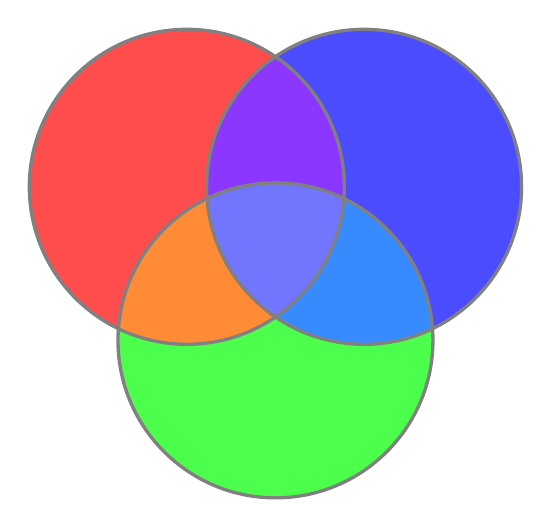
\begin{tikzpicture}
  \begin{scope}[blend group=soft light]
   \fill[blue!70!white] (30:1.3) circle (2cm);
   \fill[red!70!white] (150:1.3) circle (2cm);
   \fill[green!70!white] (270:1.3) circle (2cm);
  \end{scope}
  \draw[gray,very thick] (30:1.3) circle (2cm);
  \draw[gray,very thick] (150:1.3) circle (2cm);
  \draw[gray,very thick] (270:1.3) circle (2cm);
 \end{tikzpicture}
 \caption{Množiny $\clr{A}, \clb{B}, \clg{C}$ s neprázdným průnikem.}
 \label{fig:inkluze-exkluze-1}
\end{figure}

Budeme nyní počítat velikost sjednocení $\clr{A} \cup \clb{B} \cup \clg{C}$.

Za předpokladu, že by množiny byly disjunktní, stačilo by zkrátka sečíst
velikosti jednotlivých množin. V této situaci však započteme některé prvky
vícekrát. Stane se to proto, že když sečtu třeba $\# \clr{A} + \# \clb{B}$, tak
prvky, které leží i v $\clr{A}$ i v $\clb{B}$ (tedy ty v průniku
\textcolor[HTML]{7f33e8}{$A \cap B$}) započtu dvakrát. Na
\hyperref[fig:inkluze-exkluze-2]{obrázku níže} vidíte, kolikrát započteme který
\uv{díl} svého Vennova diagramu.

\begin{figure}[h]
 \centering
 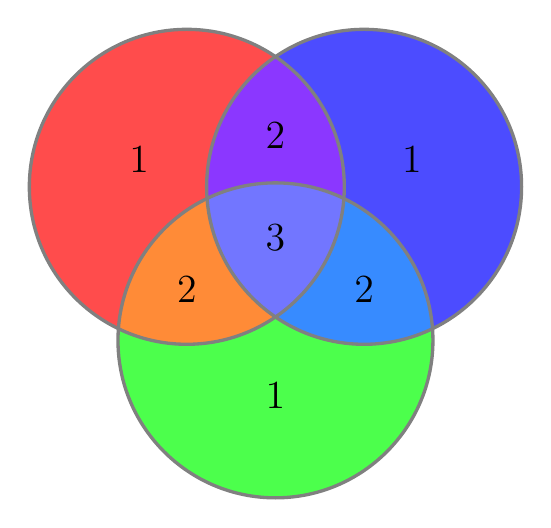
\begin{tikzpicture}
  \begin{scope}[blend group=soft light]
   \fill[blue!70!white] (30:1.3) circle (2cm);
   \fill[red!70!white] (150:1.3) circle (2cm);
   \fill[green!70!white] (270:1.3) circle (2cm);
  \end{scope}
  \draw[gray,very thick] (30:1.3) circle (2cm);
  \draw[gray,very thick] (150:1.3) circle (2cm);
  \draw[gray,very thick] (270:1.3) circle (2cm);
  
  \foreach \angle in {30,150,270} {
   \node at (\angle:2) {\Large $1$};
  }
  \foreach \angle in {90,210,330} {
   \node at (\angle:1.3) {\Large $2$};
  }
  \node at (0,0) {\Large $3$};
 \end{tikzpicture}
 \caption{Znázornění součtu $\# \clr{A} + \# \clb{B} + \# \clg{C}$.}
 \label{fig:inkluze-exkluze-2}
\end{figure}

Jak můžete vyčíst z \hyperref[fig:inkluze-exkluze-2]{obrázku}, některé průniky
jsme započítali mockrát. Černá čísla značí, kolikrát jsme každý kousek
sjednocení započetli, když jsme sečetli $\# \clr{A} + \# \clb{B} + \# \clg{C}$.
Například jsme tedy započetli každý prvek ležící v průniku
$\textcolor[HTML]{e78033}{A \cap C}$ dvakrát a každý prvek v průniku
$\textcolor[HTML]{6a6ee9}{A \cap B \cap C}$ dokonce třikrát.

Abychom situaci napravili, a započetli průnik každého páru množin jen jednou,
odečteme od součtu $\# \clr{A} + \# \clb{B} + \# \clg{C}$ velikosti všech
průniků dvou množin. Odpovídající diagram vidíte
\hyperref[fig:inkluze-exkluze-3]{níže}.

\begin{figure}[h]
 \centering
 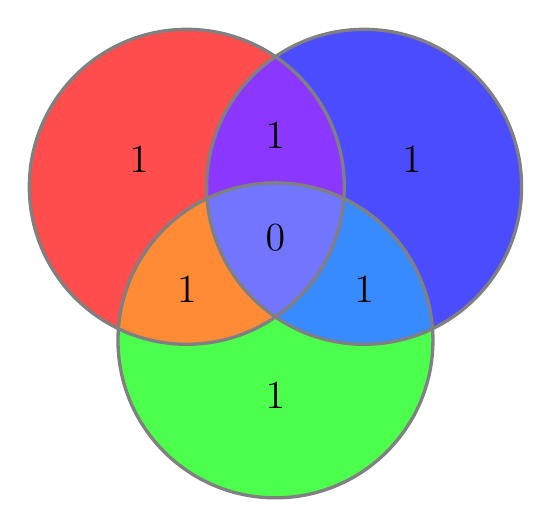
\begin{tikzpicture}
  \begin{scope}[blend group=soft light]
   \fill[blue!70!white] (30:1.3) circle (2cm);
   \fill[red!70!white] (150:1.3) circle (2cm);
   \fill[green!70!white] (270:1.3) circle (2cm);
  \end{scope}
  \draw[gray,very thick] (30:1.3) circle (2cm);
  \draw[gray,very thick] (150:1.3) circle (2cm);
  \draw[gray,very thick] (270:1.3) circle (2cm);
  
  \foreach \angle in {30,150,270} {
   \node at (\angle:2) {\Large $1$};
  }
  \foreach \angle in {90,210,330} {
   \node at (\angle:1.3) {\Large $1$};
  }
  \node at (0,0) {\Large $0$};
 \end{tikzpicture}
 \caption{Znázornění výrazu $\# \clr{A} + \# \clb{B} + \# \clg{C} - \#
 \textcolor[HTML]{7f33e8}{A \cap B} - \# \textcolor[HTML]{e78033}{A \cap C} - \#
 \textcolor[HTML]{3a87ef}{B \cap C}$.}
 \label{fig:inkluze-exkluze-3}
\end{figure}

Ovšem, nyní jsme zase odečetli třikrát průnik $\textcolor[HTML]{6a6ee9}{A \cap B
\cap C}$, protože každý prvek v $\textcolor[HTML]{6a6ee9}{A \cap B \cap C}$ leží
zároveň v $\textcolor[HTML]{7f33e8}{A \cap B}$, v $\textcolor[HTML]{e78033}{A
\cap C}$ i v $\textcolor[HTML]{3a87ef}{B \cap C}$, a ty jsme všechny odečetli.
Tedy nám z průniku $\textcolor[HTML]{6a6ee9}{A \cap B \cap C}$ žádné prvky
nezůstaly. Situaci napravíme tím, že jeho velikost přičteme zpátky. Celkově
dostaneme pro velikost sjednocení $\# A \cup B \cup C$ vzorec
\[
 \# A \cup B \cup C = \# \clr{A} + \# \clb{B} + \# \clg{C} - \#
 \textcolor[HTML]{7f33e8}{A \cap B} - \# \textcolor[HTML]{e78033}{A \cap C} - \#
 \textcolor[HTML]{3a87ef}{B \cap C} + \# \textcolor[HTML]{6a6ee9}{A \cap B \cap
 C}.
\]
Finální znázornění vidíte na
\hyperref[fig:inkluze-exkluze-4]{obrázku~\ref*{fig:inkluze-exkluze-4}}.

\begin{figure}[h]
 \centering
 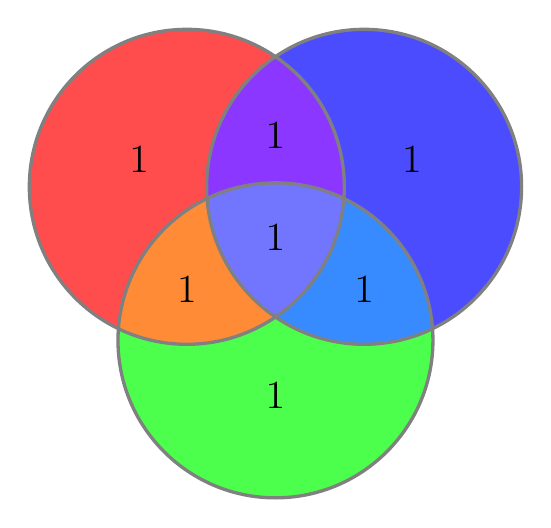
\begin{tikzpicture}
  \begin{scope}[blend group=soft light]
   \fill[blue!70!white] (30:1.3) circle (2cm);
   \fill[red!70!white] (150:1.3) circle (2cm);
   \fill[green!70!white] (270:1.3) circle (2cm);
  \end{scope}
  \draw[gray,very thick] (30:1.3) circle (2cm);
  \draw[gray,very thick] (150:1.3) circle (2cm);
  \draw[gray,very thick] (270:1.3) circle (2cm);
  
  \foreach \angle in {30,150,270} {
   \node at (\angle:2) {\Large $1$};
  }
  \foreach \angle in {90,210,330} {
   \node at (\angle:1.3) {\Large $1$};
  }
  \node at (0,0) {\Large $1$};
 \end{tikzpicture}
 \caption{Velikost sjednocení $\# A \cup B \cup C$ podle principu inkluze a
 exkluze.}
 \label{fig:inkluze-exkluze-4}
\end{figure}

Formální znění principu inkluze a exkluze dí, že tento postup funguje zcela
obecně, tedy že pokud průniky sudého počtu množin odečítám a lichého počtu
přičítám, dostanu tím velikost sjednocení.

Ještě předtím, než ho uvedeme a dokážeme, si ale určíme počet studentů
z~\hyperref[exam:inkluze-exkluze]{úvodního příkladu}. Množiny němčinářů,
španělštinářů a francouzštinářů označíme po řadě $N$, $\check{S}$ a $\check{Z}$
(jako \textbf{ž}abožrout). Ze zadání víme, že $\# N = 30, \# \check{S} = 25$ a
$\# \check{Z} = 2$. Dále víme, že $\# N \cap \check{S} = 4$, protože mezi
němčináři jsou čtyři španělštináři; podobně $\# N \cap \check{Z} = 1$ a $\#
\check{S} \cap \check{Z} = 0$. Konečně, $\# N  \cap \check{S} \cap \check{Z} =
1$. Podle principu inkluze a exkluze máme
\begin{align*}
 \# N \cup \check{S} \cup \check{Z} &= \# N + \# \check{S} + \# \check{Z} - \# N
  \cap \check{S} - \# N  \cap \check{Z} - \# \check{S} \cap \check{Z} + \# N
  \cap \check{S}  \cap \check{Z}\\
 &= 30 + 25 + 2 - 4 - 1 - 0 + 1 = 53.
\end{align*}
Celkem se tedy na Gymnáziu Growth Severní Obec učí 53 studentů cizím jazykům.

Posledním krokem, který zbývá, je umět princip inkluze a exkluze nějak rozumně
zapsat. Tohle je asi první situace, na kterou jsme narazili, kdy bez rozumného
zápisu daného tvrzení bychom se ze symbolů doslova zbláznili (hlavně v jeho
důkazu). Natvrdo napsaný říká princip inkluze a exkluze, že
\begin{align*}
 \# \bigcup_{i=1}^{n} A_i &= \# A_1 + \# A_2 + \cdots + \# A_n\\
 &- \# A_1 \cap A_2 - \# A_1 \cap A_3 - \cdots - \# A_1 \cap A_n - \# A_2
 \cap A_3 - \cdots - \# A_{n-1} \cap A_n\\
 &+ \# A_1 \cap A_2 \cap A_3 + \cdots + \# A_{n-2} \cap A_{n-1} \cap A_n +
 \cdots + (-1)^{n-1} \bigcap_{i=1}^{n} A_i.
\end{align*}
Jak sami vidíte, z tohoto zápisu je sotva (pokud vůbec) poznat, čemu se vlastně
velikost sjednocení $\bigcup_{i=1}^{n} A_i$ rovná. Musíme tento zápis
zjednodušit. Nejprve, pro každou $I \subseteq \{1,\ldots,n\}$ znamená zápis
\[
 \bigcap_{i \in I}^{} A_i
\]
průnik přesně těch množin $A_i$, jejichž indexy leží v množině $I$. Je-li tedy
např. $I = \{1,4,5\}$, pak
\[
 \bigcap_{i  \in I}^{} A_i = A_1 \cap A_4 \cap A_5.
\]
Pro extrémní případ $I = \emptyset$ dodefinujeme $\bigcap_{i \in  I}^{}A_i
\coloneqq \emptyset$, tedy prázdný průnik je prázdná množina.

Dále si rozmyslíme jednoduchý způsob, jak zapsat znaménko u každého z průniků.
Víme, že průnik sudého počtu množin má záporné znaménko a průnik lichého počtu
má kladné. Ještě jinak, když $\# I$ je sudé číslo, pak $\bigcap_{i \in  I}^{}
A_i$ musí dostat záporné znaménko, a když $\# I$ je liché číslo, tak kladné. V
matematice se pro tyto účely obvykle používá $(-1)^{k}$ pro přirozené číslo $k
\in \N$, protože $(-1)^{k}=1$, když $k$ je sudé, a $(-1)^{k} = -1$, když $k$ je
liché. To ale znamená, že výraz $\# \bigcap_{i \in  I}^{} A_i$ musí být
vynásobený číslem $(-1)^{\# I-1}$.

Už jsme skoro hotovi. Pro vyjádření $\# \bigcup_{i=1}^{n} A_i$ pomocí průniků
musíme sečíst velikosti všech průniků $k$ různých množin pro $k$ od $1$ až do
$n$ se správným znaménkem. Čili, musíme sčítat všechny výrazy $(-1)^{\# I - 1}\#
\bigcap_{i \in  I}^{} A_i$ pro všechny podmnožiny $I \subseteq \{1,\ldots,n\}$.

Předchozí diskuse nám umožňuje zapsat princip inkluze a exkluze jako rovnost
\[
 \# \bigcup_{i=1}^{n} A_i = \sum_{I \subseteq \{1,\ldots,n\}}^{} (-1)^{\# I - 1}
 \# \bigcap_{i \in  I}^{} A_i,
\]
kde symbol $\sum_{I \subseteq \{1,\ldots,n\}}^{}$ značí součet přes všechny
\textbf{podmnožiny} množiny $\{1,\ldots,n\}$.

Ještě jednou tedy princip inkluze a exkluze formulujeme jako větu.

\begin{theorem}[Princip inkluze a exkluze]
 \label{thm:princip-inkluze-a-exkluze}
 Ať $A_1,A_2,\ldots,A_n$ jsou množiny. Pak platí rovnost
 \begin{equation*}
  \label{eq:inkluze-exkluze}
  \tag{$\triangle$}
  \# \bigcup_{i=1}^{n} A_i = \sum_{I \subseteq \{1,\ldots,n\}}^{} (-1)^{\# I -
  1} \# \bigcap_{i \in  I}^{} A_i.
 \end{equation*}
\end{theorem}
\begin{proof}
 Důkaz povedeme indukcí podle $n$.

 Když $n = 1$, pak na levé straně rovnosti \eqref{eq:inkluze-exkluze} máme
 \[
  \# \bigcup_{i=1}^{1} A_i = \# A_1
 \]
 a na pravé straně
 \begin{align*}
  \sum_{I \subseteq \{1\}}^{} (-1)^{\# I - 1} \# \bigcap_{i \in  I}^{} A_i &=
  (-1)^{\#\emptyset-1} \# \bigcap_{i  \in \emptyset}^{} A_i + (-1)^{\#\{1\}-1}
  \# \bigcap_{i  \in \{1\}}^{} A_i\\
  &= (-1)^{-1} \cdot 0 + (-1)^{0} \cdot \# A_1 = \# A_1,
 \end{align*}
 protože jediné podmnožiny $\{1\}$ jsou $\emptyset$ a $\{1\}$. Čili pro $n = 1$ 
 rovnost \eqref{eq:inkluze-exkluze} platí.

 Předpokládejme nyní, že rovnost platí pro všechna čísla menší než $n$ a
 dokazujme rovnost pro $n$. Sjednocení na levé straně \eqref{eq:inkluze-exkluze}
 můžeme napsat jako
 \[
  \bigcup_{i=1}^{n} A_i = \clr{\bigcup_{i=1}^{n-1} A_i} \cup \clb{A_n}.
 \]
 Označíme si $\clr{B_1} \coloneqq \clr{\bigcup_{i=1}^{n-1} A_i}$ a $\clb{B_2}
 \coloneqq \clb{A_n}$. Podle principu inkluze a exkluze pro 2 množiny (ten
 můžeme použít z indukčního předpokladu) máme
 \[
  \# \clr{B_1} \cup \clb{B_2} = \# \clr{B_1} + \# \clb{B_2} - \# \clr{B_1} \cap
  \clb{B_2}.
 \]
 Přepsání zpět do množin $A_i$ nám dá
 \[
  \# \bigcup_{i=1}^{n} A_i= \# \clr{\bigcup_{i=1}^{n-1} A_i} \cup \clb{A_n} = \#
  \clr{\bigcup_{i=1}^{n-1} A_i} + \# \clb{A_n} - \#
  \left(\clr{\bigcup_{i=1}^{n-1} A_i} \cap \clb{A_n}\right).
 \]
 Nejprve si uvědomíme, že
 \[
  \left(\clr{\bigcup_{i=1}^{n-1} A_i}\right) \cap \clb{A_n} =
  \bigcup_{i=1}^{n-1} (\clr{A_i} \cap \clb{A_n}),
 \]
 tedy, že je to samé sjednotit množiny $\clr{A_i}$ a pak je proniknout s
 množinou $\clb{A_n}$ jako nejprve proniknout každou množinu $\clr{A_i}$ s
 množinou $\clb{A_n}$ a pak všechny ty průniky sjednotit.

 Teď můžeme (opět z indukčního předpokladu) použít princip inkluze a exkluze na
 sjednocení $\bigcup_{i=1}^{n-1} \clr{A_i}$ a zároveň na $\bigcup_{i=1}^{n-1}
 (\clr{A_i} \cap \clb{A_n})$.

 Dostaneme
 \[
  \# \bigcup_{i=1}^{n-1} \clr{A_i} = \sum_{I \subseteq \{1,\ldots,n-1\}}
  (-1)^{\# I - 1} \# \bigcap_{i \in  I}^{} \clr{A_i}
 \]
 a
 \[
  \# \bigcup_{i=1}^{n-1} (\clr{A_i} \cap \clb{A_n}) = \sum_{I \subseteq
  \{1,\ldots,n-1\}}^{} (-1)^{\# I - 1} \# \bigcap_{i \in  I}^{} (\clr{A_i} \cap
  \clb{A_n}). 
 \]
 Na jedné straně tedy máme vyjádření
 \begin{equation}
  \label{eq:ink-exk-1}
  \begin{split}
   \# \bigcup_{i=1}^{n} A_i &= \sum_{I \subseteq \{1,\ldots,n-1\}}^{} (-1)^{\# I -
   1} \# \bigcap_{i \in  I}^{} \clr{A_i} + \# \clb{A_n}\\
   &- \sum_{I \subseteq \{1,\ldots,n-1\}}^{} (-1)^{\# I - 1} \# \bigcap_{i \in
   I}^{} (\clr{A_i} \cap \clb{A_n}).
  \end{split}
 \end{equation}
 Na druhé straně potřebujeme dokázat (\textbf{ještě to nevíme!}), že
 \begin{equation}
  \label{eq:ink-exk-2}
  \# \bigcup_{i=1}^{n} A_i  \overset{?}{=} \sum_{I \subseteq \{1,\ldots,n\}}^{}
  (-1)^{\# I - 1} \# \bigcap_{i \in  I}^{} A_i.
 \end{equation}
 Porovnáváme tedy součty na pravých stranách rovností \eqref{eq:ink-exk-1} a
 \eqref{eq:ink-exk-2}. Jediný rozumný způsob, jak to udělat, je podívat se, že
 každý sčítanec v~\eqref{eq:ink-exk-2} je rovněž sčítancem v
 \eqref{eq:ink-exk-1}.

 Rozlišíme dva případy podle toho, zda podmnožina $I$ obsahuje $n$, či ne.
 \begin{enumerate}[label=(\alph*)]
  \item Ať nejprve $n \notin I$. Pak v sumě \eqref{eq:ink-exk-2} je sčítanec
   \[
    (-1)^{\# I-1} \# \bigcap_{i \in  I}^{} A_i,
   \]
   kde ten průnik neobsahuje $A_n$, protože $n \notin I$. Jenže pak je $I
   \subseteq \{1,\ldots,n-1\}$, a tedy i součet \eqref{eq:ink-exk-1} obsahuje
   ten samý sčítanec (v té úplně první sumě nahoře) se stejným znaménkem.
  \item Teď předpokládáme, že $n \in I$. Musíme rozlišit zase dva případy (xD).
   \begin{enumerate}[label=(\greek*)]
    \item $I = \{n\}$. Pak součet \eqref{eq:ink-exk-2} obsahuje sčítanec
     \[
      (-1)^{\#\{n\}-1} \# \bigcap_{i \in \{n\}}^{} A_i = \# A_n,
     \]
     který je ale i v součtu \eqref{eq:ink-exk-1} (mezi těmi dvěma sumami).
    \item $I$ obsahuje $n$ a $\# I \geq 2$. V tomto případě máme v součtu
     \eqref{eq:ink-exk-2} sčítanec
     \[
      (-1)^{\# I - 1} \# \bigcap_{i \in I}^{} A_i,
     \]
     jejž si však můžeme přepsat jako
     \begin{align*}
      (-1)^{\# I - 1} \# \bigcap_{i \in I}^{} A_i &= (-1)^{\# I - 1} \#
      \left(\bigcap_{i \in  I \setminus \{n\}}^{} \clr{A_i}\right) \cap
      \clb{A_n}\\
      &= (-1)^{\# I - 1} \# \bigcap_{i  \in I \setminus \{n\}}^{} (\clr{A_i}
      \cap \clb{A_n}),
     \end{align*}
     jelikož předpokládáme, že $n \in I$. Protože $I \setminus \{n\} \subseteq
     \{1,\ldots,n-1\}$, je v součtu \eqref{eq:ink-exk-1} (v té sumě dole)
     sčítanec
     \[
     (-1)^{\#(I \setminus \{n\}) - 1} \# \bigcap_{i  \in I \setminus \{n\}}^{}
     (\clr{A_i} \cap \clb{A_n}),
     \]
     což je v podstatě tentýž, až na znaménko. To však není problém, neboť si
     můžete všimnout, že v součtu \eqref{eq:ink-exk-1} tu druhou sumu obsahující
     všechny průniky s množinou $\clb{A_n}$ odečítám. Tedy, odpovídající
     sčítanec má ve skutečnosti znaménko $-(-1)^{\# (I \setminus \{n\})-1} =
     (-1)^{\# I - 1}$.
   \end{enumerate}
 \end{enumerate}
 Tím jsme ověřili, že součet ve vyjádření \eqref{eq:ink-exk-1} obsahuje přesně
 tytéž sčítance jako součet ve vyjádření \eqref{eq:ink-exk-2}, a tudíž se jedná
 o stejný součet. Tím je podle principu matematické indukce důkaz dokončen.
\end{proof}

Nakonec se podíváme, že
\hyperref[thm:princip-inkluze-a-exkluze]{věta~\ref*{thm:princip-inkluze-a-exkluze}}
souhlasí plně s naší intuicí v již prozkoumaném případě tří množin s neprázdným
průnikem.

\begin{example}
 Uvažme množiny $A_1,A_2,A_3$ takové, že $A_1 \cap A_2 \cap A_3 \neq \emptyset$.
 Podle \hyperref[thm:princip-inkluze-a-exkluze]{principu inkluze a exkluze}
 počítáme
 \[
  \# A_1 \cup A_2 \cup A_3 = \sum_{I \subseteq \{1,2,3\}}^{} (-1)^{\#I - 1}\#
  \bigcap_{i \in  I}^{} A_i.
 \]
 Jednoprvkové podmnožiny $\{1,2,3\}$ jsou $\{1\}, \{2\}$ a $\{3\}$. Tedy
 započteme
 \[
  (-1)^{1-1} \# A_1 + (-1)^{1-1}\# A_2 + (-1)^{1-1}\# A_3 = \# A_1 + \# A_2 + \#
  A_3.
 \]
 Ty dvouprvkové jsou $\{1,2\}, \{1,3\}$ a $\{2,3\}$. Dávají nám po řadě sčítance
 \begin{align*}
  &(-1)^{2-1}\# A_1 \cap A_2 + (-1)^{2-1}\# A_1 \cap A_3 + (-1)^{2-1}\# A_2 \cap
  A_3\\
  &= -\# A_1 \cap A_2 - \# A_1 \cap A_3 - \#A_2 \cap A_3.
 \end{align*}
 Konečně, tříprvkovou podmnožinu má $\{1,2,3\}$ jenom jednu -- sebe samu. Za tu
 si započteme
 \[
  (-1)^{3-1}\#A_1 \cap A_2 \cap A_3 = \# A_1 \cap A_2 \cap A_3.
 \]
 Když sečteme průniky přes všechny podmnožiny $\{1,2,3\}$, dostaneme
 \begin{align*}
  \# A_1 \cup A_2 \cup A_3 &= \#A_1 + \#A_2 + \#A_3\\
  &-\#A_1 \cap A_2 - \#A_1 \cap A_3 - \#A_2 \cap A_3\\
  &+ \# A_1 \cap A_2 \cap A_3,
 \end{align*}
 jak jsme očekávali.
\end{example}

Kterak káže obyčej, pár cvičení závěrem.

\begin{exercise}[zase trocha teorie čísel]
 Jeden z oblíbených a celkem rychlých rozkladů čísla na prvočísla je tzv.
 \emph{Eratosthenovo síto}.
 
 Funguje na principu vyškrtávání násobků čísel. Konkrétně, algoritmus prochází
 seznam čísel až do nějaké hranice, a kdykoli narazí na ještě neodškrtnuté
 číslo, odškrtne z tohoto seznamu všechny jeho násobky kromě něho samotného.
 Sami si rozmyslete, že tímto způsobem zůstanou ve výsledném seznamu pouze
 prvočísla.

 My si tady rozmyslíme pouze zjednodušenou verzi. Spočtěte, kolik zůstane čísel
 mezi $1$ a $1000$ potom, co vyškrtáme všechny násobky čísel $2,3,5$ a $7$.
\end{exercise}

\begin{exercise}
 Určete počet přirozených čísel menších než $100$, které nedělí druhá mocnina
 žádného přirozeného čísla (kromě $1$).
\end{exercise}

\begin{exercise}
 Kolika způsoby lze seřadit do řady 5 Čechů, 4 Maďary a 3 Rusy, aby všichni
 příslušníci jednoho národa nikdy nestáli hned za sebou?
\end{exercise}

